
%%%%%%%%%%%%%%%%%%%%%%%%%%%%%%%%%%%%%%%%%%%%%%%%%%%%%%%%
%
% Copyright (c) 2003-2010 by University of Queensland
% Earth Systems Science Computational Center (ESSCC)
% http://www.uq.edu.au/esscc
%
% Primary Business: Queensland, Australia
% Licensed under the Open Software License version 3.0
% http://www.opensource.org/licenses/osl-3.0.php
%
%%%%%%%%%%%%%%%%%%%%%%%%%%%%%%%%%%%%%%%%%%%%%%%%%%%%%%%%


\chapter{The \pyvisi Module}\label{PYVISI CHAP}
%\declaremodule{extension}{esys.pyvisi}
%\modulesynopsis{Python Visualization Interface}

\begin{Large}\strong{Warning: The Module \pyvisi is no longer supported and will be removed from future releases.}\end{Large}


\strong{\begin{Large}Warning: The Module \pyvisi is not supported under MPI        \end{Large}.}

\section{Introduction}
\pyvisi is a Python module that is used to generate 2D and 3D visualizations
for escript and its PDE solver finley. The module provides
an easy to use interface to the \VTK library (\VTKUrl) to render (generate)
surface maps and contours for scalar fields, arrows and streamlines for vector
fields, and ellipsoids for tensor fields. There are three approaches for
rendering an object. (1) Online - object is rendered on-screen with
interaction capability (i.e. zoom and rotate), (2) Offline - object is
rendered off-screen (no pop-up window) and (3) Display - object is rendered
on-screen but with no interaction capability (on-the-fly animation). All three
approaches have the option to save the rendered object as an image (e.g. jpeg)
and subsequently converting a series of images into a movie (mpeg).

The following outlines the general steps to use Pyvisi:

\begin{enumerate}
\item Create a \Scene instance - a window in which objects will be rendered on.
\item Create a data input instance (i.e. \DataCollector or \ImageReader) -
reads the source data for visualization.
\item Create a data visualization object (i.e. \Map, \Velocity, \Ellipsoid,
\Contour, \Carpet, \StreamLine, etc.) - creates a visual representation of
the source data.
\item Create a \Camera or \Light instance - controls the viewing angle and
lighting effects.
\item Render the object - using either the Online, Offline or Display approach.
\item Generate movie - converts a series of images into a movie. (optional)
\end{enumerate}
\begin{center}
\begin{math}
scene \rightarrow data \; input \rightarrow data \; visualization \rightarrow
camera \, / \, light \rightarrow render \rightarrow movie
\end{math}
\end{center}

\section{\pyvisi Classes}
The following subsections give a brief overview of the important classes
and some of their corresponding methods. Please refer to \ReferenceGuide for
full details.


%#############################################################################


\subsection{Scene Classes}
This section details the instances used to setup the viewing environment.

\subsubsection{\Scene class}

\begin{classdesc}{Scene}{renderer = Renderer.ONLINE, num_viewport = 1,
x_size = 1152, y_size = 864}
A scene is a window in which objects are to be rendered on. Only
one scene needs to be created. However, a scene may be divided into four
smaller windows called viewports (if needed). Each viewport in turn can
render a different object.
\end{classdesc}

The following are some of the methods available:
\begin{methoddesc}[Scene]{setBackground}{color}
Set the background color of the scene.
\end{methoddesc}

\begin{methoddesc}[Scene]{render}{image_name = None}
Render the object using either the Online, Offline or Display mode.
\end{methoddesc}

\subsubsection{\Camera class}

\begin{classdesc}{Camera}{scene, viewport = Viewport.SOUTH_WEST}
A camera controls the display angle of the rendered object and one is
usually created for a \Scene. However, if a \Scene has four viewports, then a
separate camera may be created for each viewport.
\end{classdesc}

The following are some of the methods available:
\begin{methoddesc}[Camera]{setFocalPoint}{position}
Set the focal point of the camera.
\end{methoddesc}

\begin{methoddesc}[Camera]{setPosition}{position}
Set the position of the camera.
\end{methoddesc}

\begin{methoddesc}[Camera]{azimuth}{angle}
Rotate the camera to the left and right. The angle parameter is in degrees.
\end{methoddesc}

\begin{methoddesc}[Camera]{elevation}{angle}
Rotate the camera up and down (angle must be between -90 and 90).
\end{methoddesc}

\begin{methoddesc}[Camera]{backView}{}
Rotate the camera to view the back of the rendered object.
\end{methoddesc}

\begin{methoddesc}[Camera]{topView}{}
Rotate the camera to view the top of the rendered object.
\end{methoddesc}

\begin{methoddesc}[Camera]{bottomView}{}
Rotate the camera to view the bottom of the rendered object.
\end{methoddesc}

\begin{methoddesc}[Camera]{leftView}{}
Rotate the camera to view the left side of the rendered object.
\end{methoddesc}

\begin{methoddesc}[Camera]{rightView}{}
Rotate the camera to view the right side of the rendered object.
\end{methoddesc}

\begin{methoddesc}[Camera]{isometricView}{}
Rotate the camera to view an isometric projection of the rendered object.
\end{methoddesc}

\begin{methoddesc}[Camera]{dolly}{distance}
Move the camera towards (greater than 1) the rendered object. However,
it is not possible to move the camera away from the rendered object with this
method.
\end{methoddesc}

\subsubsection{\Light class}

\begin{classdesc}{Light}{scene, viewport = Viewport.SOUTH_WEST}
A light controls the lighting effect for the rendered object and is set up in
a similar way to \Camera.
\end{classdesc}

The following are some of the methods available:
\begin{methoddesc}[Light]{setColor}{color}
Set the light color.
\end{methoddesc}

\begin{methoddesc}[Light]{setFocalPoint}{position}
Set the focal point of the light.
\end{methoddesc}

\begin{methoddesc}[Light]{setPosition}{position}
Set the position of the light.
\end{methoddesc}

\begin{methoddesc}[Light]{setAngle}{elevation = 0, azimuth = 0}
An alternative to set the position and focal point of the light by using
elevation and azimuth.
\end{methoddesc}


%##############################################################################


\subsection{Input Classes}
\label{INPUT SEC}
This subsection details the instances used to read and load the source data
for visualization.

\subsubsection{\DataCollector class}
\begin{classdesc}{DataCollector}{source = Source.XML}
A data collector is used to read data either from an XML file (using
\texttt{setFileName()}) or from an escript object directly (using
\texttt{setData()}). Writing XML files is expensive but has the advantage
that the results can be analyzed easily after the simulation has completed.
\end{classdesc}

The following are some of the methods available:
\begin{methoddesc}[DataCollector]{setFileName}{file_name}
Set the XML file name to read.
\end{methoddesc}

\begin{methoddesc}[DataCollector]{setData}{**args}
Create data using the \textless name\textgreater=\textless data\textgreater
pairing. The method assumes that the data is given in the appropriate format.
\end{methoddesc}

\begin{methoddesc}[DataCollector]{setActiveScalar}{scalar}
Specify the scalar field to load.
\end{methoddesc}

\begin{methoddesc}[DataCollector]{setActiveVector}{vector}
Specify the vector field to load.
\end{methoddesc}

\begin{methoddesc}[DataCollector]{setActiveTensor}{tensor}
Specify the tensor field to load.
\end{methoddesc}

\subsubsection{\ImageReader class}

\begin{classdesc}{ImageReader}{format}
An image reader is used to read data from an image in a variety of formats.
\end{classdesc}

The following is one of the methods available:
\begin{methoddesc}[ImageReader]{setImageName}{image_name}
Set the filename of the image to be loaded.
\end{methoddesc}

\subsubsection{\TextTwoD class}

\begin{classdesc}{Text2D}{scene, text, viewport = Viewport.SOUTH_WEST}
This class is used to insert two-dimensional text for annotations
(e.g. titles, authors and labels).
\end{classdesc}

The following are some of the methods available:
\begin{methoddesc}[Text2D]{setFontSize}{size}
Set the 2D text size.
\end{methoddesc}

\begin{methoddesc}[Text2D]{boldOn}{}
Use bold font style for the text.
\end{methoddesc}

\begin{methoddesc}[Text2D]{setColor}{color}
Set the color of the 2D text.
\end{methoddesc}

Including methods from \ActorTwoD.


%##############################################################################


\subsection{Data Visualization Classes}
\label{DATAVIS SEC}
This subsection details the instances used to process and manipulate the source
data. The typical usage of some of the classes is also shown. See \Sec{SAMPLEOUTPUT SEC} for sample images generated with these classes.

One point to note is that the source can either be point or cell data. If the
source is cell data, a conversion to point data may or may not be
required, in order for the object to be rendered correctly.
If a conversion is needed, the 'cell_to_point' flag (see below) must
be set to 'True', otherwise to 'False' (which is the default). On occasions, an
inaccurate object may be rendered from cell data even after conversion.

\subsubsection{\Map class}

\begin{classdesc}{Map}{scene, data_collector,
viewport = Viewport.SOUTH_WEST, lut = Lut.COLOR, cell_to_point = False,
outline = True}
Class that shows a scalar field on a domain surface. The domain surface
can either be color or gray-scale, depending on the lookup table used.
\end{classdesc}

The following are some of the methods available:\\
Methods from \ActorThreeD and \DataSetMapper.

A typical usage of \Map is shown below.

\begin{python}
"""
Author: John Ngui, john.ngui@uq.edu.au
"""

# Import the necessary modules.
from esys.pyvisi import Scene, DataCollector, Map, Camera
from esys.pyvisi.constant import *
import os

PYVISI_EXAMPLE_MESHES_PATH = "data_meshes"
PYVISI_EXAMPLE_IMAGES_PATH = "data_sample_images"
X_SIZE = 800
Y_SIZE = 800

SCALAR_FIELD_POINT_DATA = "temperature"
SCALAR_FIELD_CELL_DATA = "temperature_cell"
FILE_3D = "interior_3D.xml"
IMAGE_NAME = "map.jpg"
JPG_RENDERER = Renderer.ONLINE_JPG

# Create a Scene with four viewports.
s = Scene(renderer = JPG_RENDERER, num_viewport = 4, x_size = X_SIZE,
        y_size = Y_SIZE)

# Create a DataCollector reading from a XML file.
dc1 = DataCollector(source = Source.XML)
dc1.setFileName(file_name = os.path.join(PYVISI_EXAMPLE_MESHES_PATH, FILE_3D))
dc1.setActiveScalar(scalar = SCALAR_FIELD_POINT_DATA)

# Create a  Map for the first viewport.
m1 = Map(scene = s, data_collector = dc1, viewport = Viewport.SOUTH_WEST,
        lut = Lut.COLOR, cell_to_point = False, outline = True)
m1.setRepresentationToWireframe()

# Create a Camera for the first viewport
c1 = Camera(scene = s, viewport = Viewport.SOUTH_WEST)
c1.isometricView()

# Create a second DataCollector reading from the same XML file but specifying
# a different scalar field.
dc2 = DataCollector(source = Source.XML)
dc2.setFileName(file_name = os.path.join(PYVISI_EXAMPLE_MESHES_PATH, FILE_3D))
dc2.setActiveScalar(scalar = SCALAR_FIELD_CELL_DATA)

# Create a Map for the third viewport.
m2 = Map(scene = s, data_collector = dc2, viewport = Viewport.NORTH_EAST,
        lut = Lut.COLOR, cell_to_point = True, outline = True)

# Create a Camera for the third viewport
c2 = Camera(scene = s, viewport = Viewport.NORTH_EAST)

# Render the object.
s.render(image_name = os.path.join(PYVISI_EXAMPLE_IMAGES_PATH, IMAGE_NAME))
\end{python}

\subsubsection{\MapOnPlaneCut class}

\begin{classdesc}{MapOnPlaneCut}{scene, data_collector,
viewport = Viewport.SOUTH_WEST, lut = Lut.COLOR, cell_to_point = False,
outline = True}
This class works in a similar way to \Map, except that the result is a slice of
the scalar field produced by cutting the map with a plane. The plane can be
translated and rotated to its desired position.
\end{classdesc}

The following are some of the methods available:\\
Methods from \ActorThreeD, \Transform and \DataSetMapper.

\subsubsection{\MapOnPlaneClip class}

\begin{classdesc}{MapOnPlaneClip}{scene, data_collector,
viewport = Viewport.SOUTH_WEST, lut = Lut.COLOR, cell_to_point = False,
outline = True}
This class works in a similar way to \MapOnPlaneCut, except that the defined
plane is used to clip the scalar field.
\end{classdesc}

The following are some of the methods available:\\
Methods from \ActorThreeD, \Transform, \Clipper and \DataSetMapper.

\subsubsection{\MapOnScalarClip class}

\begin{classdesc}{MapOnScalarClip}{scene, data_collector,
viewport = Viewport.SOUTH_WEST, lut = Lut.COLOR, cell_to_point = False,
outline = True}
This class works in a similar way to \Map, except that it only shows parts of
the scalar field matching a scalar value.
\end{classdesc}

The following are some of the methods available:\\
Methods from \ActorThreeD, \Clipper and \DataSetMapper.

\subsubsection{\MapOnScalarClipWithRotation class}

\begin{classdesc}{MapOnScalarClipWithRotation}{scene, data_collector,
viewport = Viewport.SOUTH_WEST, lut = Lut.COLOR, cell_to_point = False}
This class works in a similar way to \Map except that it
shows a 2D scalar field clipped using a scalar value and subsequently
rotated around the z-axis to create a 3D looking effect. This class should
only be used with 2D data sets and NOT 3D.
\end{classdesc}

The following are some of the methods available:\\
Methods from \ActorThreeD, \Clipper, \Rotation and \DataSetMapper.

\subsubsection{\Velocity class}

\begin{classdesc}{Velocity}{scene, data_collector, arrow = Arrow.TWO_D,
color_mode = ColorMode.VECTOR, viewport = Viewport.SOUTH_WEST,
lut = Lut.COLOR, cell_to_point = False, outline = True}
This class is used to display a vector field using arrows. The arrows can
either be color or gray-scale, depending on the lookup table used. If the
arrows are colored, there are two possible coloring modes, either using vector
data or scalar data. Similarly, there are two possible types of arrows, either
two-dimensional or three-dimensional.
\end{classdesc}

The following are some of the methods available:\\
Methods from \ActorThreeD, \GlyphThreeD, \MaskPoints and \DataSetMapper.

\subsubsection{\VelocityOnPlaneCut class}

\begin{classdesc}{VelocityOnPlaneCut}{scene, data_collector,
arrow = Arrow.TWO_D, color_mode = ColorMode.VECTOR,
viewport = Viewport.SOUTH_WEST, lut = Lut.COLOR,
cell_to_point = False, outline = True}
This class works in a similar way to \MapOnPlaneCut, except that it shows a
vector field using arrows cut using a plane.
\end{classdesc}

The following are some of the methods available:\\
Methods from \ActorThreeD, \GlyphThreeD, \Transform, \MaskPoints and
\DataSetMapper.

A typical usage of \VelocityOnPlaneCut is shown below.

\begin{python}
"""
Author: John Ngui, john.ngui@uq.edu.au
"""

# Import the necessary modules
from esys.pyvisi import Scene, DataCollector, VelocityOnPlaneCut, Camera
from esys.pyvisi.constant import *
import os

PYVISI_EXAMPLE_MESHES_PATH = "data_meshes"
PYVISI_EXAMPLE_IMAGES_PATH = "data_sample_images"
X_SIZE = 400
Y_SIZE = 400

VECTOR_FIELD_CELL_DATA = "velocity"
FILE_3D = "interior_3D.xml"
IMAGE_NAME = "velocity.jpg"
JPG_RENDERER = Renderer.ONLINE_JPG

# Create a Scene.
s = Scene(renderer = JPG_RENDERER, num_viewport = 1, x_size = X_SIZE,
        y_size = Y_SIZE)

# Create a DataCollector reading from a XML file.
dc1 = DataCollector(source = Source.XML)
dc1.setFileName(file_name = os.path.join(PYVISI_EXAMPLE_MESHES_PATH, FILE_3D))
dc1.setActiveVector(vector = VECTOR_FIELD_CELL_DATA)

# Create VelocityOnPlaneCut.
vopc1 = VelocityOnPlaneCut(scene = s, data_collector = dc1,
        viewport = Viewport.SOUTH_WEST, color_mode = ColorMode.VECTOR,
        arrow = Arrow.THREE_D, lut = Lut.COLOR, cell_to_point = False,
        outline = True)
vopc1.setScaleFactor(scale_factor = 0.5)
vopc1.setPlaneToXY(offset = 0.5)
vopc1.setRatio(2)
vopc1.randomOn()

# Create a Camera.
c1 = Camera(scene = s, viewport = Viewport.SOUTH_WEST)
c1.isometricView()
c1.elevation(angle = -20)

# Render the object.
s.render(image_name = os.path.join(PYVISI_EXAMPLE_IMAGES_PATH, IMAGE_NAME))
\end{python}

\subsubsection{\VelocityOnPlaneClip class}

\begin{classdesc}{VelocityOnPlaneClip}{scene, data_collector,
arrow = Arrow.TWO_D, color_mode = ColorMode.VECTOR,
viewport = Viewport.SOUTH_WEST, lut = Lut.COLOR,
cell_to_point = False, online = True}
This class works in a similar way to \MapOnPlaneClip, except that it shows a
vector field using arrows clipped using a plane.
\end{classdesc}

The following are some of the methods available:\\
Methods from \ActorThreeD, \GlyphThreeD, \Transform, \Clipper,
\MaskPoints and \DataSetMapper.

\subsubsection{\Ellipsoid class}

\begin{classdesc}{Ellipsoid}{scene, data_collector,
viewport = Viewport = SOUTH_WEST, lut = Lut.COLOR, cell_to_point = False,
outline = True}
Class that shows a tensor field using ellipsoids. The ellipsoids can either be
color or gray-scale, depending on the lookup table used.
\end{classdesc}

The following are some of the methods available:\\
Methods from \ActorThreeD, \Sphere, \TensorGlyph, \MaskPoints and
\DataSetMapper.

\subsubsection{\EllipsoidOnPlaneCut class}

\begin{classdesc}{EllipsoidOnPlaneCut}{scene, data_collector,
viewport = Viewport.SOUTH_WEST, lut = Lut.COLOR, cell_to_point = False,
outline = True}
This class works in a similar way to \MapOnPlaneCut, except that it shows
a tensor field using ellipsoids cut using a plane.
\end{classdesc}

The following are some of the methods available:\\
Methods from \ActorThreeD, \Sphere, \TensorGlyph, \Transform,
\MaskPoints and \DataSetMapper.

\subsubsection{\EllipsoidOnPlaneClip class}

\begin{classdesc}{EllipsoidOnPlaneClip}{scene, data_collector,
viewport = Viewport.SOUTH_WEST, lut = Lut.COLOR, cell_to_point = False,
outline = True}
This class works in a similar way to \MapOnPlaneClip, except that it shows a
tensor field using ellipsoids clipped using a plane.
\end{classdesc}

The following are some of the methods available:\\
Methods from \ActorThreeD, \Sphere, \TensorGlyph, \Transform, \Clipper,
\MaskPoints and \DataSetMapper.

A typical usage of \EllipsoidOnPlaneClip is shown below.

\begin{python}
"""
Author: John Ngui, john.ngui@uq.edu.au
"""

# Import the necessary modules
from esys.pyvisi import Scene, DataCollector, EllipsoidOnPlaneClip, Camera
from esys.pyvisi.constant import *
import os

PYVISI_EXAMPLE_MESHES_PATH = "data_meshes"
PYVISI_EXAMPLE_IMAGES_PATH = "data_sample_images"
X_SIZE = 400
Y_SIZE = 400

TENSOR_FIELD_CELL_DATA = "stress_cell"
FILE_3D = "interior_3D.xml"
IMAGE_NAME = "ellipsoid.jpg"
JPG_RENDERER = Renderer.ONLINE_JPG

# Create a Scene.
s = Scene(renderer = JPG_RENDERER, num_viewport = 1, x_size = X_SIZE,
        y_size = Y_SIZE)

# Create a DataCollector reading from a XML file.
dc1 = DataCollector(source = Source.XML)
dc1.setFileName(file_name = os.path.join(PYVISI_EXAMPLE_MESHES_PATH, FILE_3D))
dc1.setActiveTensor(tensor = TENSOR_FIELD_CELL_DATA)

# Create an EllipsoidOnPlaneClip.
eopc1 = EllipsoidOnPlaneClip(scene = s, data_collector = dc1,
        viewport = Viewport.SOUTH_WEST, lut = Lut.COLOR, cell_to_point = True,
        outline = True)
eopc1.setPlaneToXY()
eopc1.setScaleFactor(scale_factor = 0.2)
eopc1.rotateX(angle = 10)

# Create a Camera.
c1 = Camera(scene = s, viewport = Viewport.SOUTH_WEST)
c1.bottomView()
c1.azimuth(angle = -90)
c1.elevation(angle = 10)

# Render the object.
s.render(image_name = os.path.join(PYVISI_EXAMPLE_IMAGES_PATH, IMAGE_NAME))
\end{python}

\subsubsection{\Contour class}

\begin{classdesc}{Contour}{scene, data_collector,
viewport = Viewport.SOUTH_WEST, lut = Lut.COLOR, cell_to_point = False,
outline = True}
Class that shows a scalar field using contour surfaces. The contour surfaces
can either be color or gray-scale, depending on the lookup table used. This
class can also be used to generate isosurfaces.
\end{classdesc}

The following are some of the methods available:\\
Methods from \ActorThreeD, \ContourModule and \DataSetMapper.

A typical usage of \Contour is shown below.

\begin{python}
"""
Author: John Ngui, john.ngui@uq.edu.au
"""

# Import the necessary modules
from esys.pyvisi import Scene, DataCollector, Contour, Camera
from esys.pyvisi.constant import *
import os

PYVISI_EXAMPLE_MESHES_PATH = "data_meshes"
PYVISI_EXAMPLE_IMAGES_PATH = "data_sample_images"
X_SIZE = 400
Y_SIZE = 400

SCALAR_FIELD_POINT_DATA = "temperature"
FILE_3D = "interior_3D.xml"
IMAGE_NAME = "contour.jpg"
JPG_RENDERER = Renderer.ONLINE_JPG

# Create a Scene.
s = Scene(renderer = JPG_RENDERER, num_viewport = 1, x_size = X_SIZE,
        y_size = Y_SIZE)

# Create a DataCollector reading a XML file.
dc1 = DataCollector(source = Source.XML)
dc1.setFileName(file_name = os.path.join(PYVISI_EXAMPLE_MESHES_PATH, FILE_3D))
dc1.setActiveScalar(scalar = SCALAR_FIELD_POINT_DATA)

# Create three contours.
ctr1 = Contour(scene = s, data_collector = dc1, viewport = Viewport.SOUTH_WEST,
        lut = Lut.COLOR, cell_to_point = False, outline = True)
ctr1.generateContours(contours = 3)

# Create a Camera.
cam1 = Camera(scene = s, viewport = Viewport.SOUTH_WEST)
cam1.elevation(angle = -40)

# Render the object.
s.render(image_name = os.path.join(PYVISI_EXAMPLE_IMAGES_PATH, IMAGE_NAME))
\end{python}

\subsubsection{\ContourOnPlaneCut class}

\begin{classdesc}{ContourOnPlaneCut}{scene, data_collector,
viewport = Viewport.SOUTH_WEST, lut = Lut.COLOR, cell_to_point = False,
outline = True}
This class works in a similar way to \MapOnPlaneCut, except that it shows a
scalar field using contour surfaces cut using a plane.
\end{classdesc}

The following are some of the methods available:\\
Methods from \ActorThreeD, \ContourModule, \Transform and \DataSetMapper.

\subsubsection{\ContourOnPlaneClip class}

\begin{classdesc}{ContourOnPlaneClip}{scene, data_collector,
viewport = Viewport.SOUTH_WEST, lut = Lut.COLOR, cell_to_point = False,
outline = True}
This class works in a similar way to \MapOnPlaneClip, except that it shows a
scalar field using contour surfaces clipped using a plane.
\end{classdesc}

The following are some of the methods available:\\
Methods from \ActorThreeD, \ContourModule, \Transform, \Clipper and
\DataSetMapper.

\subsubsection{\StreamLine class}

\begin{classdesc}{StreamLine}{scene, data_collector,
viewport = Viewport.SOUTH_WEST, color_mode = ColorMode.VECTOR, lut = Lut.COLOR,
cell_to_point = False, outline = True}
Class that shows the direction of particles of a vector field using streamlines.
The streamlines can either be color or gray-scale, depending on the lookup
table used. If the streamlines are colored, there are two possible coloring
modes, either using vector data or scalar data.
\end{classdesc}

The following are some of the methods available:\\
Methods from \ActorThreeD, \PointSource, \StreamLineModule, \Tube and
\DataSetMapper.

A typical usage of \StreamLine is shown below.

\begin{python}
"""
Author: John Ngui, john.ngui@uq.edu.au
"""

# Import the necessary modules.
from esys.pyvisi import Scene, DataCollector, StreamLine, Camera
from esys.pyvisi.constant import *
import os

PYVISI_EXAMPLE_MESHES_PATH = "data_meshes"
PYVISI_EXAMPLE_IMAGES_PATH = "data_sample_images"
X_SIZE = 400
Y_SIZE = 400

VECTOR_FIELD_CELL_DATA = "temperature"
FILE_3D = "interior_3D.xml"
IMAGE_NAME = "streamline.jpg"
JPG_RENDERER = Renderer.ONLINE_JPG

# Create a Scene.
s = Scene(renderer = JPG_RENDERER, num_viewport = 1, x_size = X_SIZE,
        y_size = Y_SIZE)

# Create a DataCollector reading from a XML file.
dc1 = DataCollector(source = Source.XML)
dc1.setFileName(file_name = os.path.join(PYVISI_EXAMPLE_MESHES_PATH, FILE_3D))

# Create streamlines.
sl1 = StreamLine(scene = s, data_collector = dc1,
        viewport = Viewport.SOUTH_WEST, color_mode = ColorMode.SCALAR,
        lut = Lut.COLOR, cell_to_point = False, outline = True)
sl1.setTubeRadius(radius = 0.02)
sl1.setTubeNumberOfSides(3)
sl1.setTubeRadiusToVaryByVector()
sl1.setPointSourceRadius(0.9)

# Create a Camera.
c1 = Camera(scene = s, viewport = Viewport.SOUTH_WEST)
c1.isometricView()

# Render the object.
s.render(image_name = os.path.join(PYVISI_EXAMPLE_IMAGES_PATH, IMAGE_NAME))
\end{python}

\subsubsection{\Carpet class}

\begin{classdesc}{Carpet}{scene, data_collector,
viewport = Viewport.Viewport.SOUTH_WEST, warp_mode = WarpMode.SCALAR,
lut = Lut.COLOR, cell_to_point = False, outline = True}
This class works in a similar way to \MapOnPlaneCut, except that it shows a
scalar field cut on a plane and deformed (warped) along the normal. The
plane can either be color or gray-scale, depending on the lookup table used.
Similarly, the plane can be deformed either using scalar data or vector data.
\end{classdesc}

The following are some of the methods available:\\
Methods from \ActorThreeD, \Warp, \Transform and \DataSetMapper.

A typical usage of \Carpet is shown below.

\begin{python}
"""
Author: John Ngui, john.ngui@uq.edu.au
"""

# Import the necessary modules.
from esys.pyvisi import Scene, DataCollector, Carpet, Camera
from esys.pyvisi.constant import *
import os

PYVISI_EXAMPLE_MESHES_PATH = "data_meshes"
PYVISI_EXAMPLE_IMAGES_PATH = "data_sample_images"
X_SIZE = 400
Y_SIZE = 400

SCALAR_FIELD_CELL_DATA = "temperature_cell"
FILE_3D = "interior_3D.xml"
IMAGE_NAME = "carpet.jpg"
JPG_RENDERER = Renderer.ONLINE_JPG

# Create a Scene.
s = Scene(renderer = JPG_RENDERER, num_viewport = 1, x_size = X_SIZE,
        y_size = Y_SIZE)

# Create a DataCollector reading from a XML file.
dc1 = DataCollector(source = Source.XML)
dc1.setFileName(file_name = os.path.join(PYVISI_EXAMPLE_MESHES_PATH, FILE_3D))
dc1.setActiveScalar(scalar = SCALAR_FIELD_CELL_DATA)

# Create a Carpet.
cpt1 = Carpet(scene = s, data_collector = dc1, viewport = Viewport.SOUTH_WEST,
        warp_mode = WarpMode.SCALAR, lut = Lut.COLOR, cell_to_point = True,
        outline = True)
cpt1.setPlaneToXY(0.2)
cpt1.setScaleFactor(1.9)

# Create a Camera.
c1 = Camera(scene = s, viewport = Viewport.SOUTH_WEST)
c1.isometricView()

# Render the object.
s.render(image_name = os.path.join(PYVISI_EXAMPLE_IMAGES_PATH, IMAGE_NAME))
\end{python}

\subsubsection{\Legend class}

\begin{classdesc}{Legend}{scene, data_collector,
viewport = Viewport.SOUTH_WEST, lut = Lut.COLOR, legend = LegendType.SCALAR}
Class that shows a scalar field on a domain surface. The domain surface
can either be color or gray-scale, depending on the lookup table used
\end{classdesc}

The following are some of the methods available:\\
Methods from \ActorThreeD, \ScalarBar and \DataSetMapper.

\subsubsection{\Rectangle class}

\begin{classdesc}{Rectangle}{scene, viewport = Viewport.SOUTH_WEST}
Class that generates a rectangle box.
\end{classdesc}

The following are some of the methods available:\\
Methods from \ActorThreeD, \CubeSource and \DataSetMapper.

\subsubsection{\Image class}

\begin{classdesc}{Image}{scene, image_reader, viewport = Viewport.SOUTH_WEST}
Class that displays an image which can be scaled (upwards and downwards) and
has interaction capability. The image can also be translated and rotated along
the X, Y and Z axes. One of the most common use of this feature is pasting an
image on a surface map.
\end{classdesc}

The following are some of the methods available:\\
Methods from \ActorThreeD, \PlaneSource and \Transform.

A typical usage of \Image is shown below.

\begin{python}
"""
Author: John Ngui, john.ngui@uq.edu.au
"""

# Import the necessary modules.
from esys.pyvisi import Scene, DataCollector, Map, ImageReader, Image, Camera
from esys.pyvisi import GlobalPosition
from esys.pyvisi.constant import *
import os

PYVISI_EXAMPLE_MESHES_PATH = "data_meshes"
PYVISI_EXAMPLE_IMAGES_PATH = "data_sample_images"
X_SIZE = 400
Y_SIZE = 400

SCALAR_FIELD_POINT_DATA = "temperature"
FILE_3D = "interior_3D.xml"
LOAD_IMAGE_NAME = "flinders.jpg"
SAVE_IMAGE_NAME = "image.jpg"
JPG_RENDERER = Renderer.ONLINE_JPG

# Create a Scene.
s = Scene(renderer = JPG_RENDERER, num_viewport = 1, x_size = X_SIZE,
        y_size = Y_SIZE)

# Create a DataCollector reading from a XML file.
dc1 = DataCollector(source = Source.XML)
dc1.setFileName(file_name = os.path.join(PYVISI_EXAMPLE_MESHES_PATH, FILE_3D))

# Create a Map.
m1 = Map(scene = s, data_collector = dc1, viewport = Viewport.SOUTH_WEST,
        lut = Lut.COLOR, cell_to_point = False, outline = True)
m1.setOpacity(0.3)

# Create an ImageReader (in place of DataCollector).
ir = ImageReader(ImageFormat.JPG)
ir.setImageName(image_name =  os.path.join(PYVISI_EXAMPLE_MESHES_PATH, \
        LOAD_IMAGE_NAME))

# Create an Image.
i = Image(scene = s, image_reader = ir, viewport = Viewport.SOUTH_WEST)
i.setOpacity(opacity = 0.9)
i.translate(0,0,-1)
i.setPoint1(GlobalPosition(2,0,0))
i.setPoint2(GlobalPosition(0,2,0))

# Create a Camera.
c1 = Camera(scene = s, viewport = Viewport.SOUTH_WEST)

# Render the image.
s.render(image_name = os.path.join(PYVISI_EXAMPLE_IMAGES_PATH, SAVE_IMAGE_NAME))
\end{python}

\subsubsection{\Logo class}

\begin{classdesc}{Logo}{scene, image_reader, viewport = Viewport.SOUTH_WEST}
Class that displays a static image, in particular a logo
(e.g. company symbol) and has NO interaction capability. The position and size
of the logo can be specified.
\end{classdesc}

The following are some of the methods available:\\
Methods from \ImageReslice and \ActorTwoD.

\subsubsection{\Movie class}

\begin{classdesc}{Movie}{parameter_file = "make_movie"}
This class is used to create movies out of a series of images. The parameter
specifies the name of a file that will contain the required information for the
'ppmtompeg' command which is used to generate the movie.
\end{classdesc}

The following are some of the methods available:\\
\begin{methoddesc}[Movie]{imageRange}{input_directory, first_image, last_image}
Use this method to specify that the movie is to be generated from image files
with filenames in a certain range (e.g. 'image000.jpg' to 'image050.jpg').
\end{methoddesc}

\begin{methoddesc}[Movie]{imageList}{input_directory, image_list}
Use this method to specify a list of arbitrary image filenames from which the
movie is to be generated.
\end{methoddesc}

\begin{methoddesc}[Movie]{makeMovie}{movie}
Generate the movie with the specified filename.
\end{methoddesc}

A typical usage of \Movie is shown below.

\begin{python}
"""
Author: John Ngui, john.ngui@uq.edu.au
"""

# Import the necessary modules.
from esys.pyvisi import Scene, DataCollector, Map, Camera, Velocity, Legend
from esys.pyvisi import Movie, LocalPosition
from esys.pyvisi.constant import *
import os

PYVISI_EXAMPLE_MESHES_PATH = "data_meshes"
PYVISI_EXAMPLE_IMAGES_PATH = "data_sample_images"
X_SIZE = 800
Y_SIZE = 800

SCALAR_FIELD_POINT_DATA = "temp"
FILE_2D = "tempvel-"
IMAGE_NAME = "movie"
JPG_RENDERER = Renderer.OFFLINE_JPG

# Create a Scene.
s = Scene(renderer = JPG_RENDERER, num_viewport = 1, x_size = X_SIZE,
        y_size = Y_SIZE)

# Create a DataCollector reading from a XML file.
dc1 = DataCollector(source = Source.XML)
dc1.setActiveScalar(scalar = SCALAR_FIELD_POINT_DATA)

# Create a Map.
m1 = Map(scene = s, data_collector = dc1,
        viewport = Viewport.SOUTH_WEST, lut = Lut.COLOR, cell_to_point = False,
        outline = True)

# Create a Camera.
cam1 = Camera(scene = s, viewport = Viewport.SOUTH_WEST)

# Create a movie.
mov = Movie()
lst = []

# Read in one file one after another and render the object.
for i in range(938, 949):
    dc1.setFileName(file_name =  os.path.join(PYVISI_EXAMPLE_MESHES_PATH, \
	        FILE_2D + "%06d.vtu") % i)

    s.render(image_name = os.path.join(PYVISI_EXAMPLE_IMAGES_PATH, \
            IMAGE_NAME + "%06d.jpg" % i))

    lst.append(IMAGE_NAME + "%06d.jpg" % i)

# Images (first and last inclusive) from which the movie is to be generated.
mov.imageRange(input_directory = PYVISI_EXAMPLE_IMAGES_PATH,
        first_image = IMAGE_NAME + "000938.jpg",
        last_image = IMAGE_NAME + "000948.jpg")

# Alternatively, a list of images can be specified.
#mov.imageList(input_directory = PYVISI_EXAMPLE_IMAGES_PATH, image_list = lst)

# Generate the movie.
mov.makeMovie(os.path.join(PYVISI_EXAMPLE_IMAGES_PATH, "movie.mpg"))
\end{python}


%##############################################################################


\subsection{Coordinate Classes}
This subsection details the instances used to position rendered objects.

\subsubsection{\LocalPosition class}

\begin{classdesc}{LocalPosition}{x_coor, y_coor}
Class that defines a position (X and Y) in the local 2D coordinate system.
\end{classdesc}

\subsubsection{\GlobalPosition class}

\begin{classdesc}{GlobalPosition}{x_coor, y_coor, z_coor}
Class that defines a position (X, Y and Z) in the global 3D coordinate system.
\end{classdesc}


%##############################################################################


\subsection{Supporting Classes}
This subsection details the supporting classes and their corresponding methods
inherited by the input (see \Sec{INPUT SEC}) and data
visualization classes (see \Sec{DATAVIS SEC}).

\subsubsection{\ActorThreeD class}
Class that defines a 3D actor. \\

The following are some of the methods available:

\begin{methoddesc}[Actor3D]{setOpacity}{opacity}
Set the opacity (transparency) of the 3D actor.
\end{methoddesc}

\begin{methoddesc}[Actor3D]{setColor}{color}
Set the color of the 3D actor.
\end{methoddesc}

\begin{methoddesc}[Actor3D]{setRepresentationToWireframe}{}
Set the representation of the 3D actor to wireframe.
\end{methoddesc}

\subsubsection{\ActorTwoD class}
Class that defines a 2D actor. \\

The following are some of the methods available:

\begin{methoddesc}[Actor2D]{setPosition}{position}
Set the position (XY) of the 2D actor. Default position is the lower left hand
corner of the window / viewport.
\end{methoddesc}

\subsubsection{\Clipper class}
Class that defines a clipper. \\

The following are some of the methods available:

\begin{methoddesc}[Clipper]{setInsideOutOn}{}
Clips one side of the rendered object.
\end{methoddesc}

\begin{methoddesc}[Clipper]{setInsideOutOff}{}
Clips the other side of the rendered object.
\end{methoddesc}

\begin{methoddesc}[Clipper]{setClipValue}{value}
Set the scalar clip value (instead of using a plane) for the clipper.
\end{methoddesc}

\subsubsection{\ContourModule class}
Class that defines the contour module. \\

The following are some of the methods available:

\begin{methoddesc}[ContourModule]{generateContours}{contours = None,
lower_range = None, upper_range = None}
Generate the specified number of contours within the specified range.
In order to generate a single isosurface, the 'lower_range' and 'upper_range'
must be set to the same value.
\end{methoddesc}

\subsubsection{\GlyphThreeD class}
Class that defines 3D glyphs. \\

The following are some of the methods available:

\begin{methoddesc}[Glyph3D]{setScaleModeByVector}{}
Set the 3D glyph to scale according to the vector data.
\end{methoddesc}

\begin{methoddesc}[Glyph3D]{setScaleModeByScalar}{}
Set the 3D glyph to scale according to the scalar data.
\end{methoddesc}

\begin{methoddesc}[Glyph3D]{setScaleFactor}{scale_factor}
Set the 3D glyph scale factor.
\end{methoddesc}

\subsubsection{\TensorGlyph class}
Class that defines tensor glyphs. \\

The following are some of the methods available:

\begin{methoddesc}[TensorGlyph]{setScaleFactor}{scale_factor}
Set the scale factor for the tensor glyph.
\end{methoddesc}

\begin{methoddesc}[TensorGlyph]{setMaxScaleFactor}{max_scale_factor}
Set the maximum allowable scale factor for the tensor glyph.
\end{methoddesc}

\subsubsection{\PlaneSource class}
Class that defines a plane source. A plane source is defined by an origin
and two other points, which form the axes (X and Y). \\

The following are some of the methods available:

\begin{methoddesc}[PlaneSource]{setOrigin}{position}
Set the origin of the plane source.
\end{methoddesc}

\begin{methoddesc}[PlaneSource]{setPoint1}{position}
Set the first point from the origin of the plane source.
\end{methoddesc}

\begin{methoddesc}[PlaneSource]{setPoint2}{position}
Set the second point from the origin of the plane source.
\end{methoddesc}

\subsubsection{\PointSource class}
Class that defines the source (location) to generate points. The points are
generated within the radius of a sphere. \\

The following are some of the methods available:

\begin{methoddesc}[PointSource]{setPointSourceRadius}{radius}
Set the radius of the sphere.
\end{methoddesc}

\begin{methoddesc}[PointSource]{setPointSourceCenter}{center}
Set the center of the sphere.
\end{methoddesc}

\begin{methoddesc}[PointSource]{setPointSourceNumberOfPoints}{points}
Set the number of points to generate within the sphere (the larger the
number of points, the more streamlines are generated).
\end{methoddesc}

\subsubsection{\Sphere class}
Class that defines a sphere. \\

The following are some of the methods available:

\begin{methoddesc}[Sphere]{setThetaResolution}{resolution}
Set the theta resolution of the sphere.
\end{methoddesc}

\begin{methoddesc}[Sphere]{setPhiResolution}{resolution}
Set the phi resolution of the sphere.
\end{methoddesc}

\subsubsection{\StreamLineModule class}
Class that defines the streamline module. \\

The following are some of the methods available:

\begin{methoddesc}[StreamLineModule]{setMaximumPropagationTime}{time}
Set the maximum length of the streamline expressed in elapsed time.
\end{methoddesc}

\begin{methoddesc}[StreamLineModule]{setIntegrationToBothDirections}{}
Set the integration to occur both sides: forward (where the streamline
goes) and backward (where the streamline came from).
\end{methoddesc}

\subsubsection{\Transform class}
Class that defines the orientation of planes. \\

The following are some of the methods available:

\begin{methoddesc}[Transform]{translate}{x_offset, y_offset, z_offset}
Translate the rendered object along the x, y and z-axes.
\end{methoddesc}

\begin{methoddesc}[Transform]{rotateX}{angle}
Rotate the plane around the x-axis.
\end{methoddesc}

\begin{methoddesc}[Transform]{rotateY}{angle}
Rotate the plane around the y-axis.
\end{methoddesc}

\begin{methoddesc}[Transform]{rotateZ}{angle}
Rotate the plane around the z-axis.
\end{methoddesc}

\begin{methoddesc}[Transform]{setPlaneToXY}{offset = 0}
Set the plane orthogonal to the z-axis.
\end{methoddesc}

\begin{methoddesc}[Transform]{setPlaneToYZ}{offset = 0}
Set the plane orthogonal to the x-axis.
\end{methoddesc}

\begin{methoddesc}[Transform]{setPlaneToXZ}{offset = 0}
Set the plane orthogonal to the y-axis.
\end{methoddesc}

\subsubsection{\Tube class}
Class that defines the tube wrapped around the streamlines. \\

The following are some of the methods available:

\begin{methoddesc}[Tube]{setTubeRadius}{radius}
Set the radius of the tube.
\end{methoddesc}

\begin{methoddesc}[Tube]{setTubeRadiusToVaryByVector}{}
Set the radius of the tube to vary by vector data.
\end{methoddesc}

\begin{methoddesc}[Tube]{setTubeRadiusToVaryByScalar}{}
Set the radius of the tube to vary by scalar data.
\end{methoddesc}

\subsubsection{\Warp class}
Class that defines the deformation of a scalar field. \\

The following are some of the methods available:

\begin{methoddesc}[Warp]{setScaleFactor}{scale_factor}
Set the displacement scale factor.
\end{methoddesc}

\subsubsection{\MaskPoints class}
Class that defines masking of points. This is useful to prevent the
rendered object from being cluttered with arrows or ellipsoids. \\

The following are some of the methods available:

\begin{methoddesc}[MaskPoints]{setRatio}{ratio}
Mask every n'th point.
\end{methoddesc}

\begin{methoddesc}[MaskPoints]{randomOn}{}
Enables randomization of the points selected for masking.
\end{methoddesc}

\subsubsection{\ScalarBar class}
Class that defines a scalar bar. \\

The following are some of the methods available:

\begin{methoddesc}[ScalarBar]{setTitle}{title}
Set the title of the scalar bar.
\end{methoddesc}

\begin{methoddesc}[ScalarBar]{setPosition}{position}
Set the local position of the scalar bar.
\end{methoddesc}

\begin{methoddesc}[ScalarBar]{setOrientationToHorizontal}{}
Set the orientation of the scalar bar to horizontal.
\end{methoddesc}

\begin{methoddesc}[ScalarBar]{setOrientationToVertical}{}
Set the orientation of the scalar bar to vertical.
\end{methoddesc}

\begin{methoddesc}[ScalarBar]{setHeight}{height}
Set the height of the scalar bar.
\end{methoddesc}

\begin{methoddesc}[ScalarBar]{setWidth}{width}
Set the width of the scalar bar.
\end{methoddesc}

\begin{methoddesc}[ScalarBar]{setLabelColor}{color}
Set the color of the scalar bar's label.
\end{methoddesc}

\begin{methoddesc}[ScalarBar]{setTitleColor}{color}
Set the color of the scalar bar's title.
\end{methoddesc}

\subsubsection{\ImageReslice class}
Class that defines an image reslice which is used to resize static
(no interaction capability) images (i.e. logo). \\

The following are some of the methods available:

\begin{methoddesc}[ImageReslice]{setSize}{size}
Set the size factor of the image. The value must be between 0 and 2.
Size 1 (one) keeps the image in its original size (which is the default).
\end{methoddesc}

\subsubsection{\DataSetMapper class}
Class that defines a data set mapper. \\

The following are some of the methods available:

\begin{methoddesc}[DataSetMapper]{setScalarRange}{lower_range, upper_range}
Set the minimum and maximum scalar range for the data set mapper. This
method is called when the range has been specified by the user.
Therefore, the scalar range read from the source will be ignored.
\end{methoddesc}

\subsubsection{\CubeSource class}
Class that defines a cube source. The center of the cube source defines
the point from which the cube is to be generated and the X, Y
and Z lengths define the length of the cube from the center point. If
X length is 3, then the X length to the left and right of the center
point is 1.5 respectively.\\

The following are some of the methods available:

\begin{methoddesc}[CubeSource]{setCenter}{center}
Set the cube source center.
\end{methoddesc}

\begin{methoddesc}[CubeSource]{setXLength}{length}
Set the cube source length along the x-axis.
\end{methoddesc}

\begin{methoddesc}[CubeSource]{setYLength}{length}
Set the cube source length along the y-axis.
\end{methoddesc}

\begin{methoddesc}[CubeSource]{setZLength}{length}
Set the cube source length along the z-axis.
\end{methoddesc}

\subsubsection{\Rotation class}
Class that sweeps 2D data around the z-axis to create a 3D looking effect. \\

The following are some of the methods available:

\begin{methoddesc}[Rotation]{setResolution}{resolution}
Set the resolution of the sweep for the rotation, which controls the
number of intermediate points.
\end{methoddesc}

\begin{methoddesc}[Rotation]{setAngle}{angle}
Set the angle of rotation.
\end{methoddesc}


% #############################################################################


\section{More Examples}
This section provides examples for some common tasks.

\subsection{Reading a Series of Files}
The following script shows how to generate images from a time series using
two data sources.

\begin{python}
"""
Author: John Ngui, john.ngui@uq.edu.au
"""

# Import the necessary modules.
from esys.pyvisi import Scene, DataCollector, Contour, Camera
from esys.pyvisi.constant import *
import os

PYVISI_EXAMPLE_MESHES_PATH = "data_meshes"
PYVISI_EXAMPLE_IMAGES_PATH = "data_sample_images"
X_SIZE = 400
Y_SIZE = 300

SCALAR_FIELD_POINT_DATA_1 = "lava"
SCALAR_FIELD_POINT_DATA_2 = "talus"
FILE_2D = "phi_talus_lava."

IMAGE_NAME = "seriesofreads"
JPG_RENDERER = Renderer.ONLINE_JPG

# Create a Scene.
s = Scene(renderer = JPG_RENDERER, num_viewport = 1, x_size = X_SIZE,
        y_size = Y_SIZE)

# Create a DataCollector reading from an XML file.
dc1 = DataCollector(source = Source.XML)
dc1.setActiveScalar(scalar = SCALAR_FIELD_POINT_DATA_1)

# Create a Contour.
mosc1 = Contour(scene = s, data_collector = dc1,
        viewport = Viewport.SOUTH_WEST, lut = Lut.COLOR, cell_to_point = False,
        outline = True)
mosc1.generateContours(0)

# Create a second DataCollector reading from the same XML file
# but specifying a different scalar field.
dc2 = DataCollector(source = Source.XML)
dc2.setActiveScalar(scalar = SCALAR_FIELD_POINT_DATA_2)

# Create a second Contour.
mosc2 = Contour(scene = s, data_collector = dc2,
        viewport = Viewport.SOUTH_WEST, lut = Lut.COLOR, cell_to_point = False,
        outline = True)
mosc2.generateContours(0)

# Create a Camera.
cam1 = Camera(scene = s, viewport = Viewport.SOUTH_WEST)

# Read in one file after another and render the object.
for i in range(99, 104):
    dc1.setFileName(file_name =  os.path.join(PYVISI_EXAMPLE_MESHES_PATH, \
	        FILE_2D + "%04d.vtu") % i)
    dc2.setFileName(file_name =  os.path.join(PYVISI_EXAMPLE_MESHES_PATH, \
            FILE_2D + "%04d.vtu") % i)

    s.render(image_name = os.path.join(PYVISI_EXAMPLE_IMAGES_PATH, \
            IMAGE_NAME + "%04d.jpg") % i)
\end{python}

\subsection{Creating Slices of a Data Source}
The following script shows how to save a series of images that slice the
data at different points by gradually translating the cut plane.

\begin{python}
"""
Author: John Ngui, john.ngui@uq.edu.au
"""

# Import the necessary modules.
from esys.pyvisi import Scene, DataCollector, MapOnPlaneCut, Camera
from esys.pyvisi.constant import *
import os

PYVISI_EXAMPLE_MESHES_PATH = "data_meshes"
PYVISI_EXAMPLE_IMAGES_PATH = "data_sample_images"
X_SIZE = 400
Y_SIZE = 400

SCALAR_FIELD_POINT_DATA = "temperature"
FILE_3D = "interior_3D.xml"
IMAGE_NAME = "seriesofcuts"
JPG_RENDERER = Renderer.ONLINE_JPG

# Create a Scene.
s = Scene(renderer = JPG_RENDERER, num_viewport = 1, x_size = X_SIZE,
        y_size = Y_SIZE)

# Create a DataCollector reading from an XML file.
dc1 = DataCollector(source = Source.XML)
dc1.setFileName(file_name = os.path.join(PYVISI_EXAMPLE_MESHES_PATH, FILE_3D))
dc1.setActiveScalar(scalar = SCALAR_FIELD_POINT_DATA)

# Create a MapOnPlaneCut.
mopc1 = MapOnPlaneCut(scene = s, data_collector = dc1,
        viewport = Viewport.SOUTH_WEST, lut = Lut.COLOR, cell_to_point = False,
        outline = True)
mopc1.setPlaneToYZ(offset = 0.1)

# Create a Camera.
c1 = Camera(scene = s, viewport = Viewport.SOUTH_WEST)
c1.isometricView()

# Render the object with multiple cuts using a series of translations.
for i in range(0, 5):
    s.render(image_name = os.path.join(PYVISI_EXAMPLE_IMAGES_PATH, IMAGE_NAME +
			"%02d.jpg") % i)
    mopc1.translate(0.6,0,0)
\end{python}

\subsection{Reading Data Directly from escript Objects}
The following script shows how to combine Pyvisi code with escript code to
generate visualizations on the fly.

\begin{python}
"""
Author: Lutz Gross, l.gross@uq.edu.au
Author: John Ngui, john.ngui@uq.edu.au
"""

# Import the necessary modules.
from esys.escript import *
from esys.escript.linearPDEs import LinearPDE
from esys.finley import Rectangle
from esys.pyvisi import Scene, DataCollector, Map, Camera
from esys.pyvisi.constant import *
import os

PYVISI_EXAMPLE_IMAGES_PATH = "data_sample_images"
X_SIZE = 400
Y_SIZE = 400
JPG_RENDERER = Renderer.ONLINE_JPG

#... set some parameters ...
xc = [0.02,0.002]
r = 0.001
qc = 50.e6
Tref = 0.
rhocp = 2.6e6
eta = 75.
kappa = 240.
tend = 5.
# initialize time, time step size and counter ...
t=0
h=0.1
i=0

# generate domain ...
mydomain = Rectangle(l0=0.05, l1=0.01, n0=250, n1=50)
# open PDE ...
mypde = LinearPDE(mydomain)
mypde.setSymmetryOn()
mypde.setValue(A=kappa*kronecker(mydomain), D=rhocp/h, d=eta, y=eta*Tref)
# set heat source: ...
x = mydomain.getX()
qH = qc*whereNegative(length(x-xc)-r)

# set initial temperature ....
T=Tref

# Create a Scene.
s = Scene(renderer = JPG_RENDERER, x_size = X_SIZE, y_size = Y_SIZE)

# Create a DataCollector reading directly from escript objects.
dc = DataCollector(source = Source.ESCRIPT)

# Create a Map.
m = Map(scene = s, data_collector = dc, \
        viewport = Viewport.SOUTH_WEST, lut = Lut.COLOR, \
        cell_to_point = False, outline = True)

# Create a Camera.
c = Camera(scene = s, viewport = Viewport.SOUTH_WEST)

# start iteration
while t < 0.4:
      i += 1
      t += h
      mypde.setValue(Y=qH+rhocp/h*T)
      T = mypde.getSolution()

      dc.setData(temp = T)

      # Render the object.
      s.render(image_name = os.path.join(PYVISI_EXAMPLE_IMAGES_PATH, \
              "diffusion%02d.jpg") % i)
\end{python}

\newpage

\section{Useful Keys}
This section lists keyboard shortcuts available when interacting with rendered
objects using the Online approach.

\begin{table}[ht]
\begin{center}
\begin{tabular}{| c | p{12cm} |}
\hline
\textbf{Key} & \textbf{Description} \\ \hline
Keypress 'c' / 'a' & Toggle between the camera ('c') and object ('a')  mode. In
camera mode, mouse events affect the camera position and focal point. In
object mode, mouse events affect the rendered object's element (i.e.
cut surface map, clipped velocity field, streamline, etc) that is under the
mouse pointer.\\ \hline
Mouse button 1 & Rotate the camera around its focal point (if in camera mode)
or rotate the rendered object's element (if in object mode).\\ \hline
Mouse button 2 & Pan the camera (if in camera mode) or translate the rendered
object's element (if in object mode). \\ \hline
Mouse button 3 & Zoom the camera (if in camera mode) or scale the rendered
object's element (if in object mode). \\ \hline
Keypress 3 & Toggle the render window in and out of stereo mode. By default,
red-blue stereo pairs are created. \\ \hline
Keypress 'e' / 'q' & Exit the application if only one file is to be read, or
read and display the next file if multiple files are to be read. \\ \hline
Keypress 's' & Modify the representation of the rendered object to surfaces.
\\ \hline
Keypress 'w' & Modify the representation of the rendered object to wireframe.
\\ \hline
Keypress 'r' & Reset the position of the rendered object to the center.
\\ \hline
\end{tabular}
\caption{Useful keys in Online render mode}
\end{center}
\end{table}


% ############################################################################


\newpage
\renewcommand{\textfraction}{0.06} % force first table to stay with the text
\section{Sample Output}
\label{SAMPLEOUTPUT SEC}
This section shows sample images produced with the various classes of Pyvisi.
The source code to produce these images is included in the Pyvisi distribution.
%
\begin{table}[hb]
\begin{tabular}{c c c}
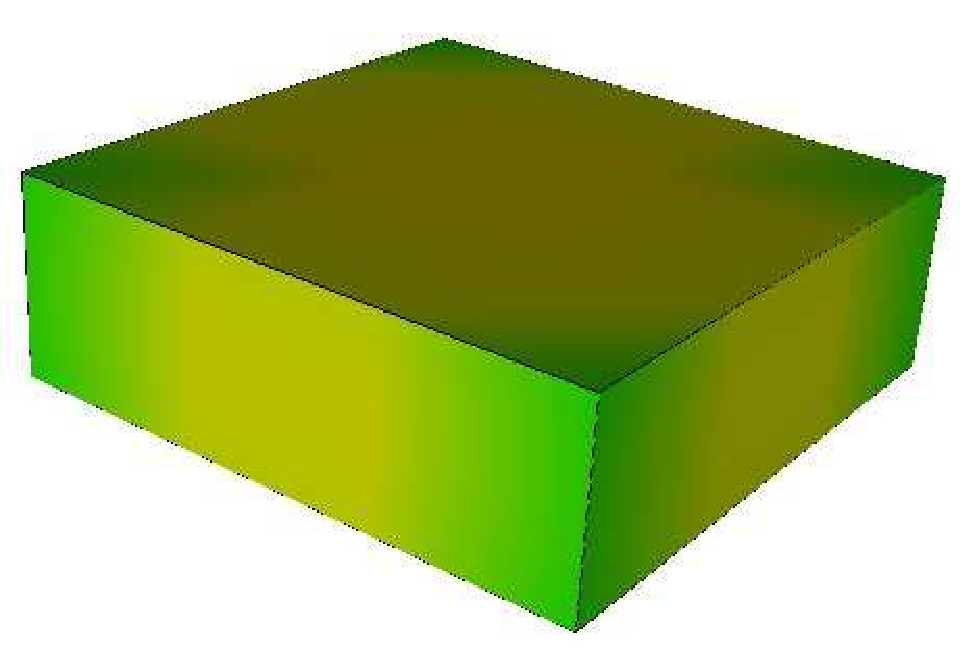
\includegraphics[width=\thumbnailwidth]{Map} &
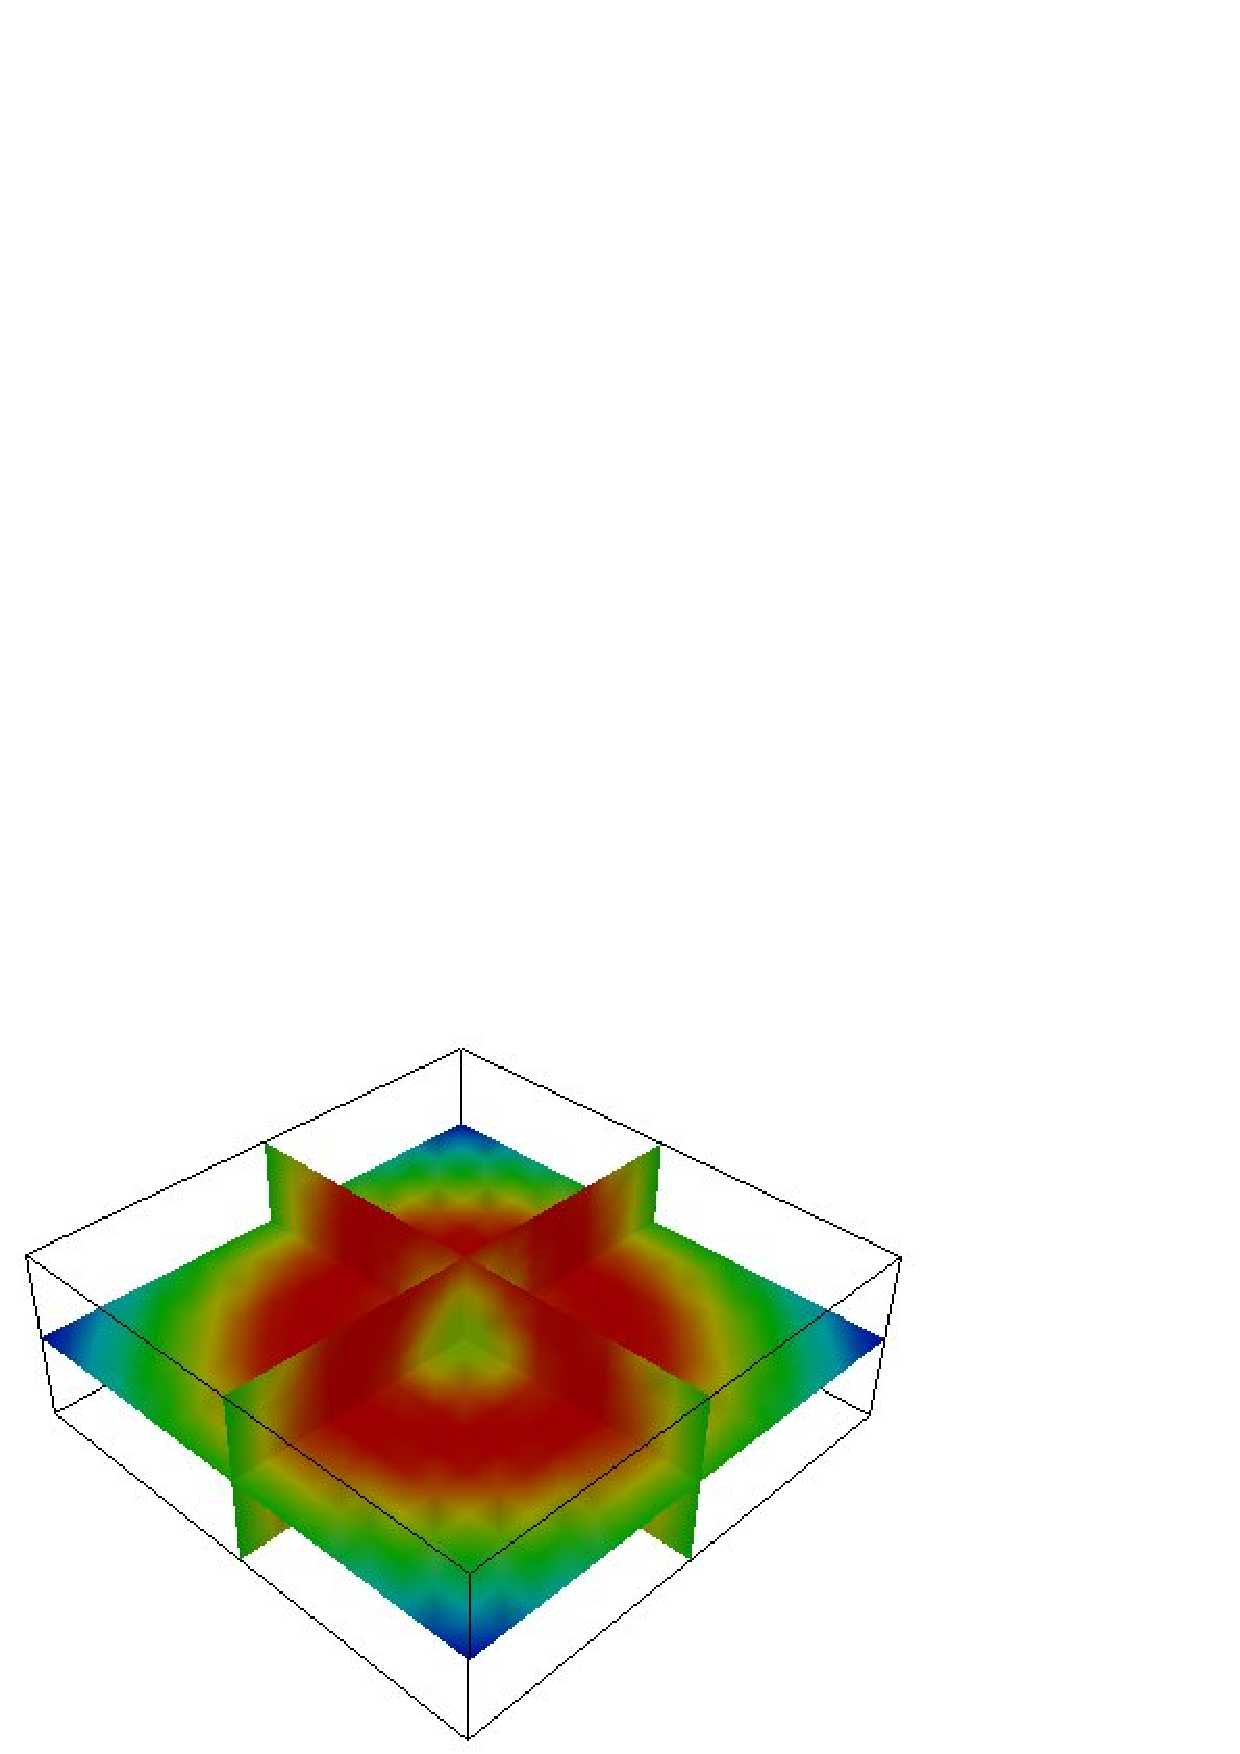
\includegraphics[width=\thumbnailwidth]{MapOnPlaneCut} &
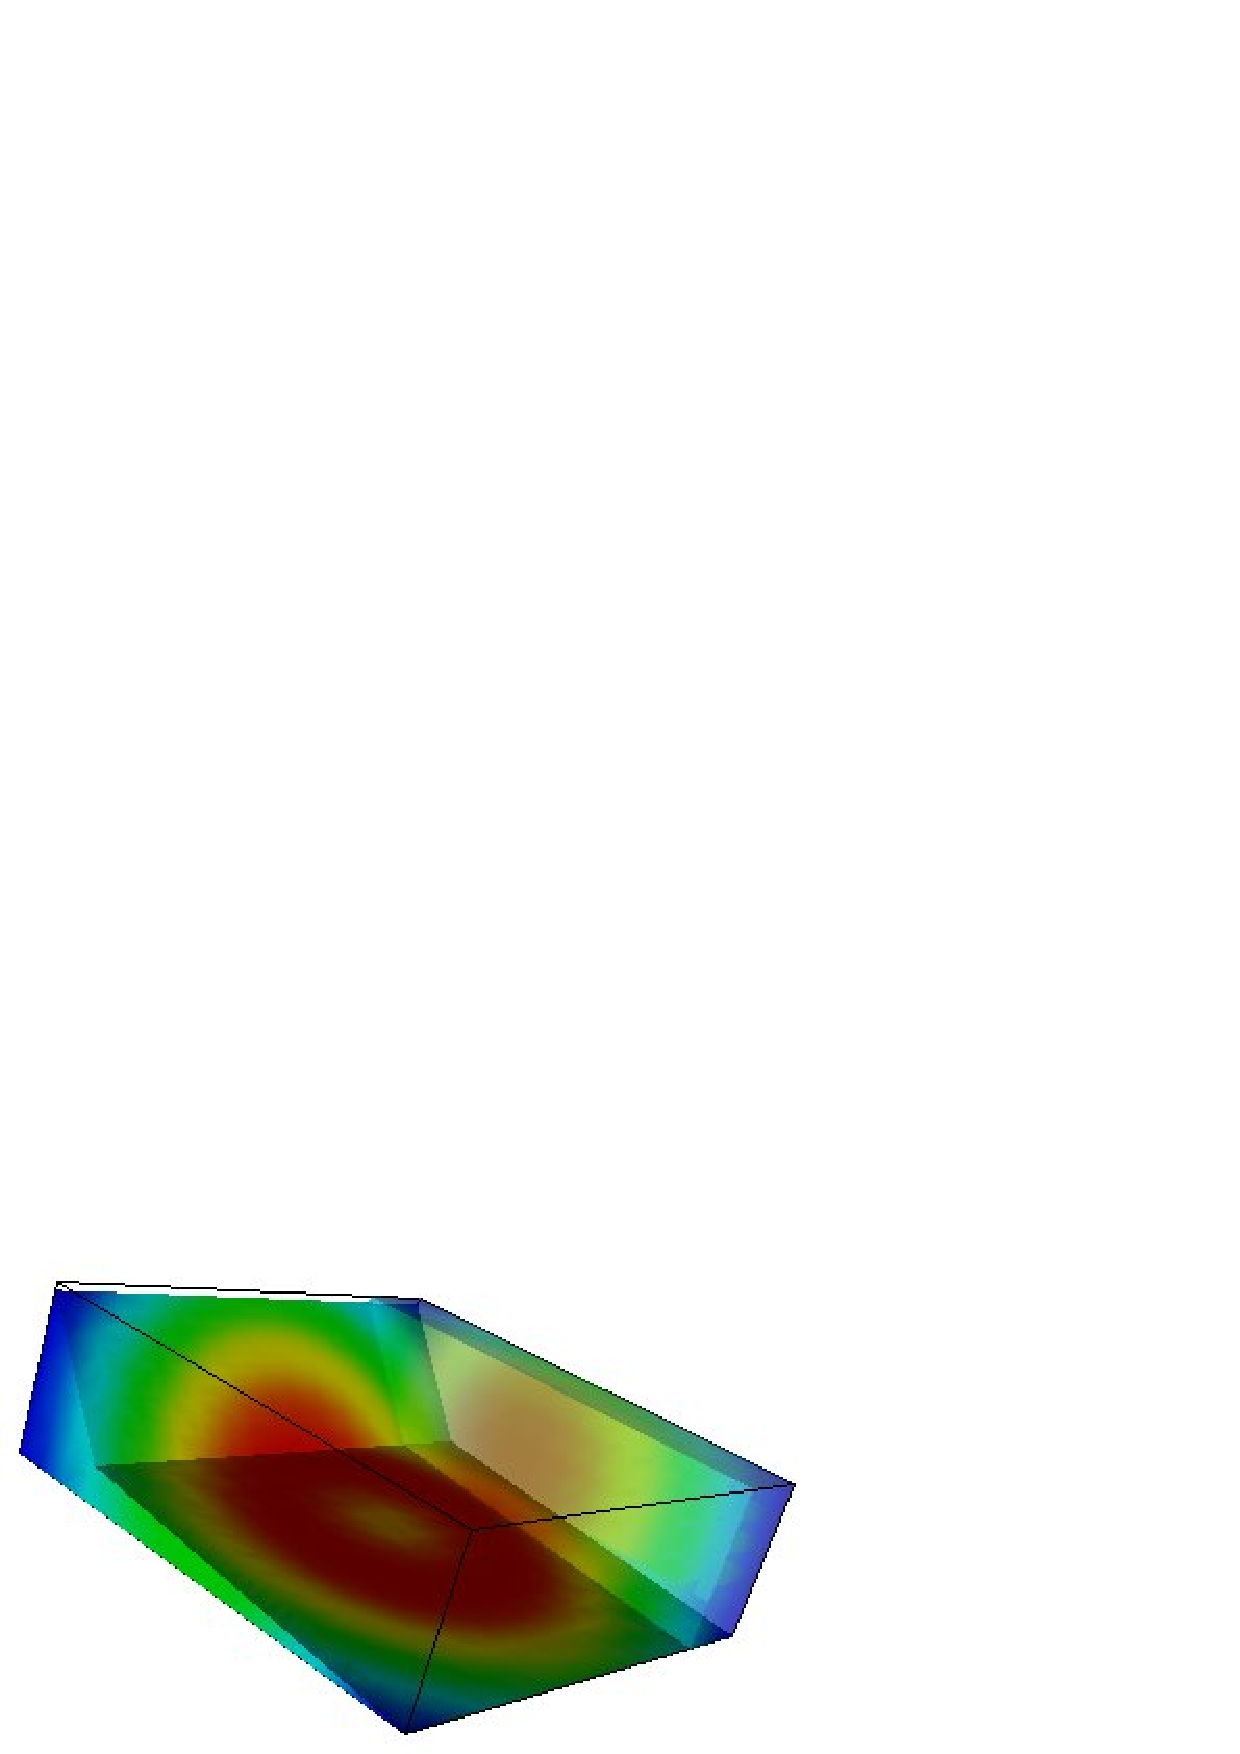
\includegraphics[width=\thumbnailwidth]{MapOnPlaneClip} \\
Map & MapOnPlaneCut & MapOnPlaneClip \\
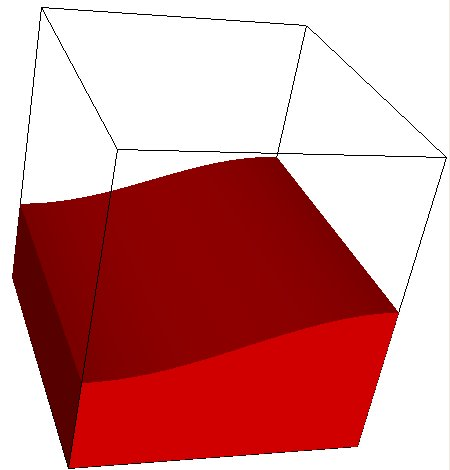
\includegraphics[width=\thumbnailwidth]{MapOnScalarClip} &
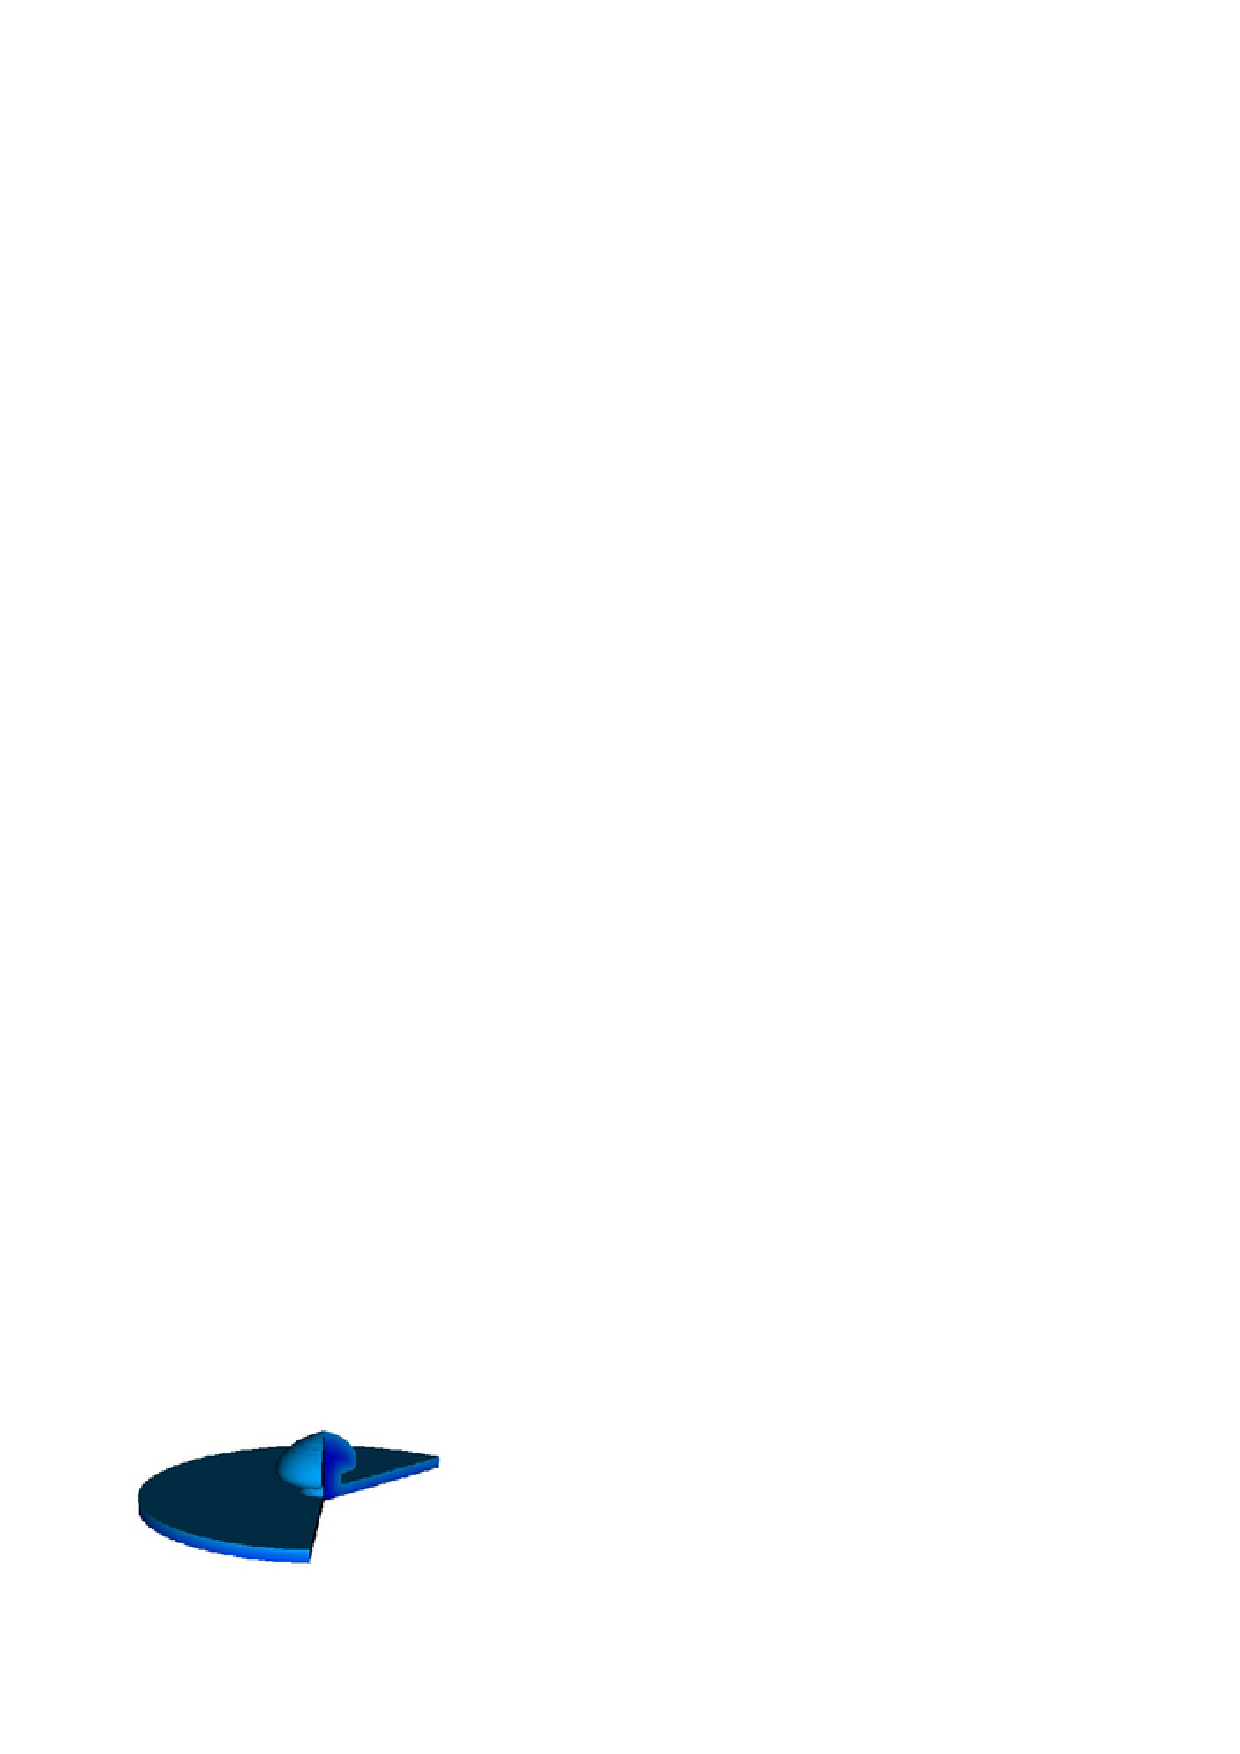
\includegraphics[width=\thumbnailwidth]{MapOnScalarClipWithRotation} &
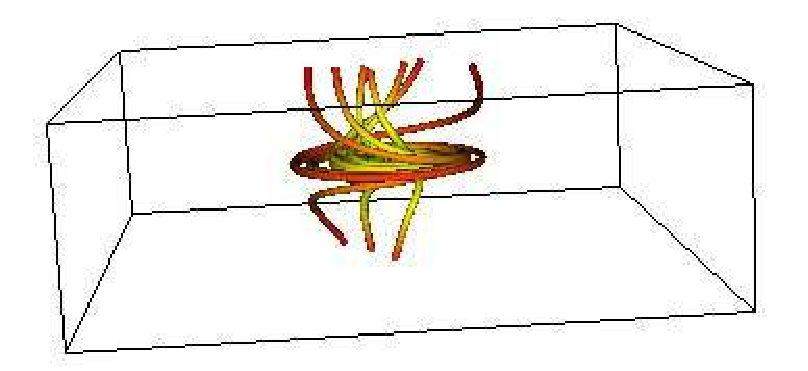
\includegraphics[width=\thumbnailwidth]{StreamLine} \\
MapOnScalarClip & MapOnScalarClipWithRotation & Streamline \\ \\ \\
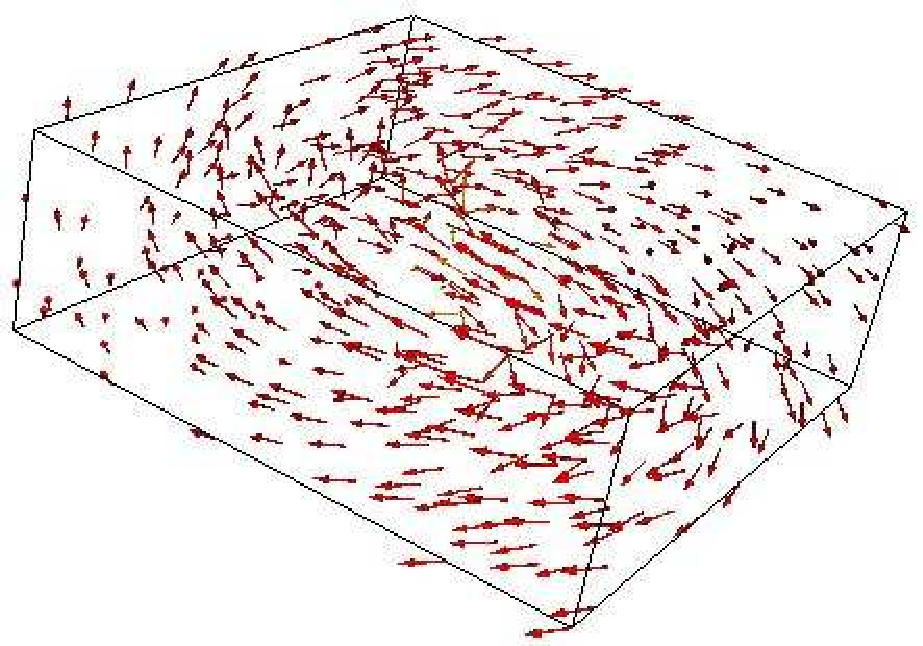
\includegraphics[width=\thumbnailwidth]{Velocity} &
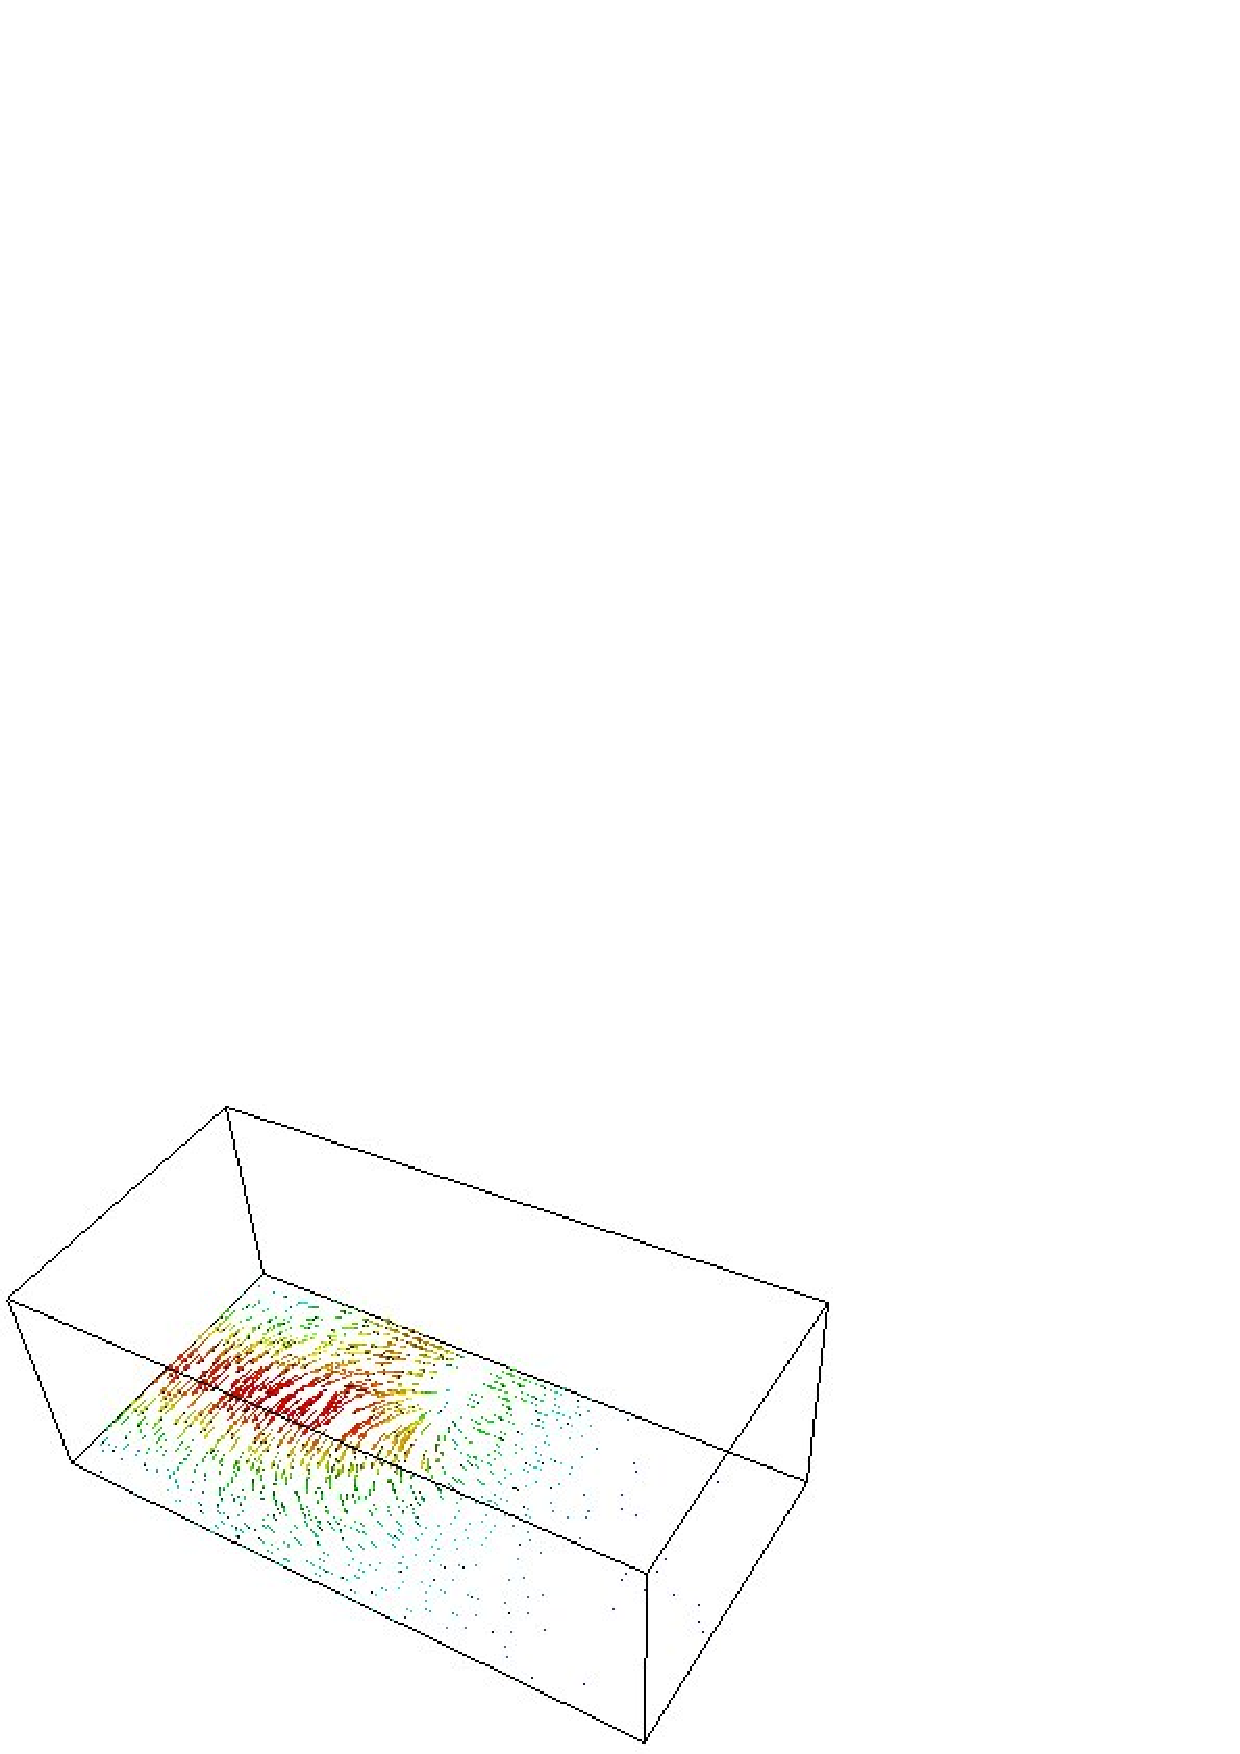
\includegraphics[width=\thumbnailwidth]{VelocityOnPlaneCut} &
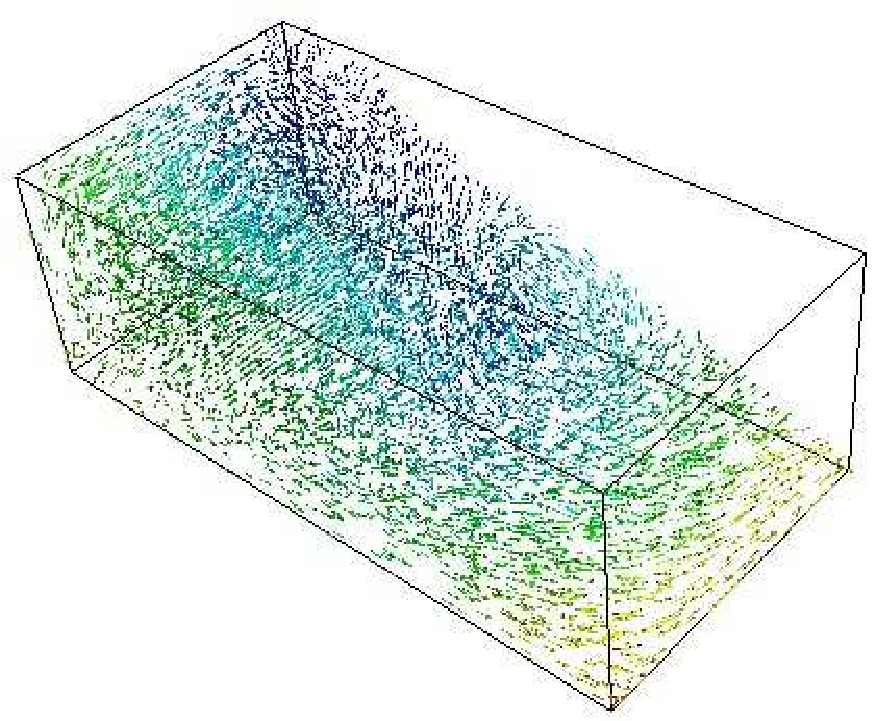
\includegraphics[width=\thumbnailwidth]{VelocityOnPlaneClip} \\
Velocity & VelocityOnPlaneCut & VelocityOnPlaneClip \\ \\ \\
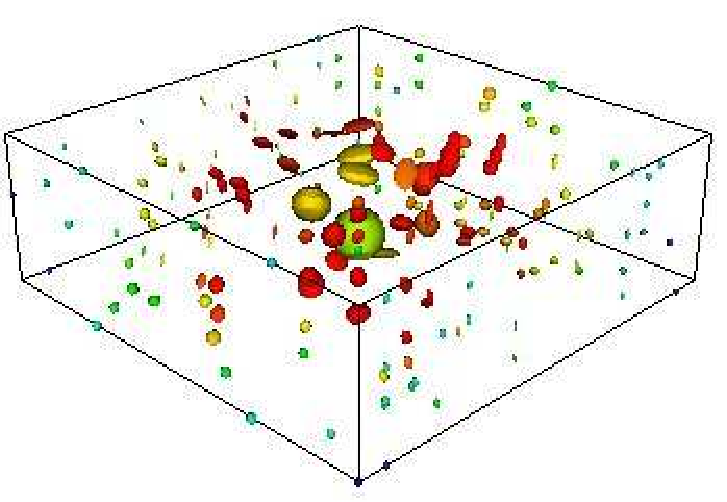
\includegraphics[width=\thumbnailwidth]{Ellipsoid} &
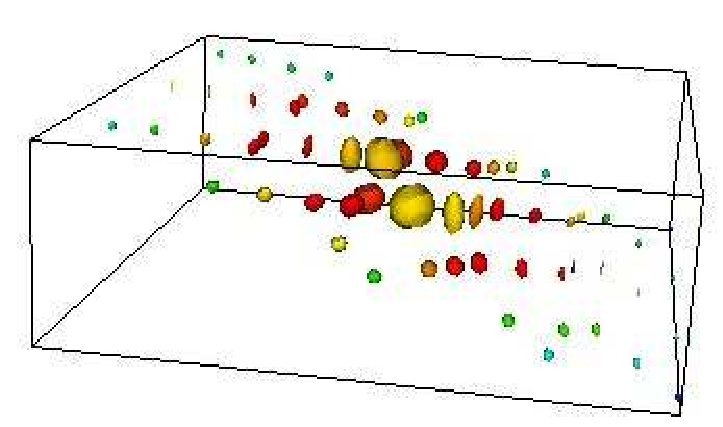
\includegraphics[width=\thumbnailwidth]{EllipsoidOnPlaneCut} &
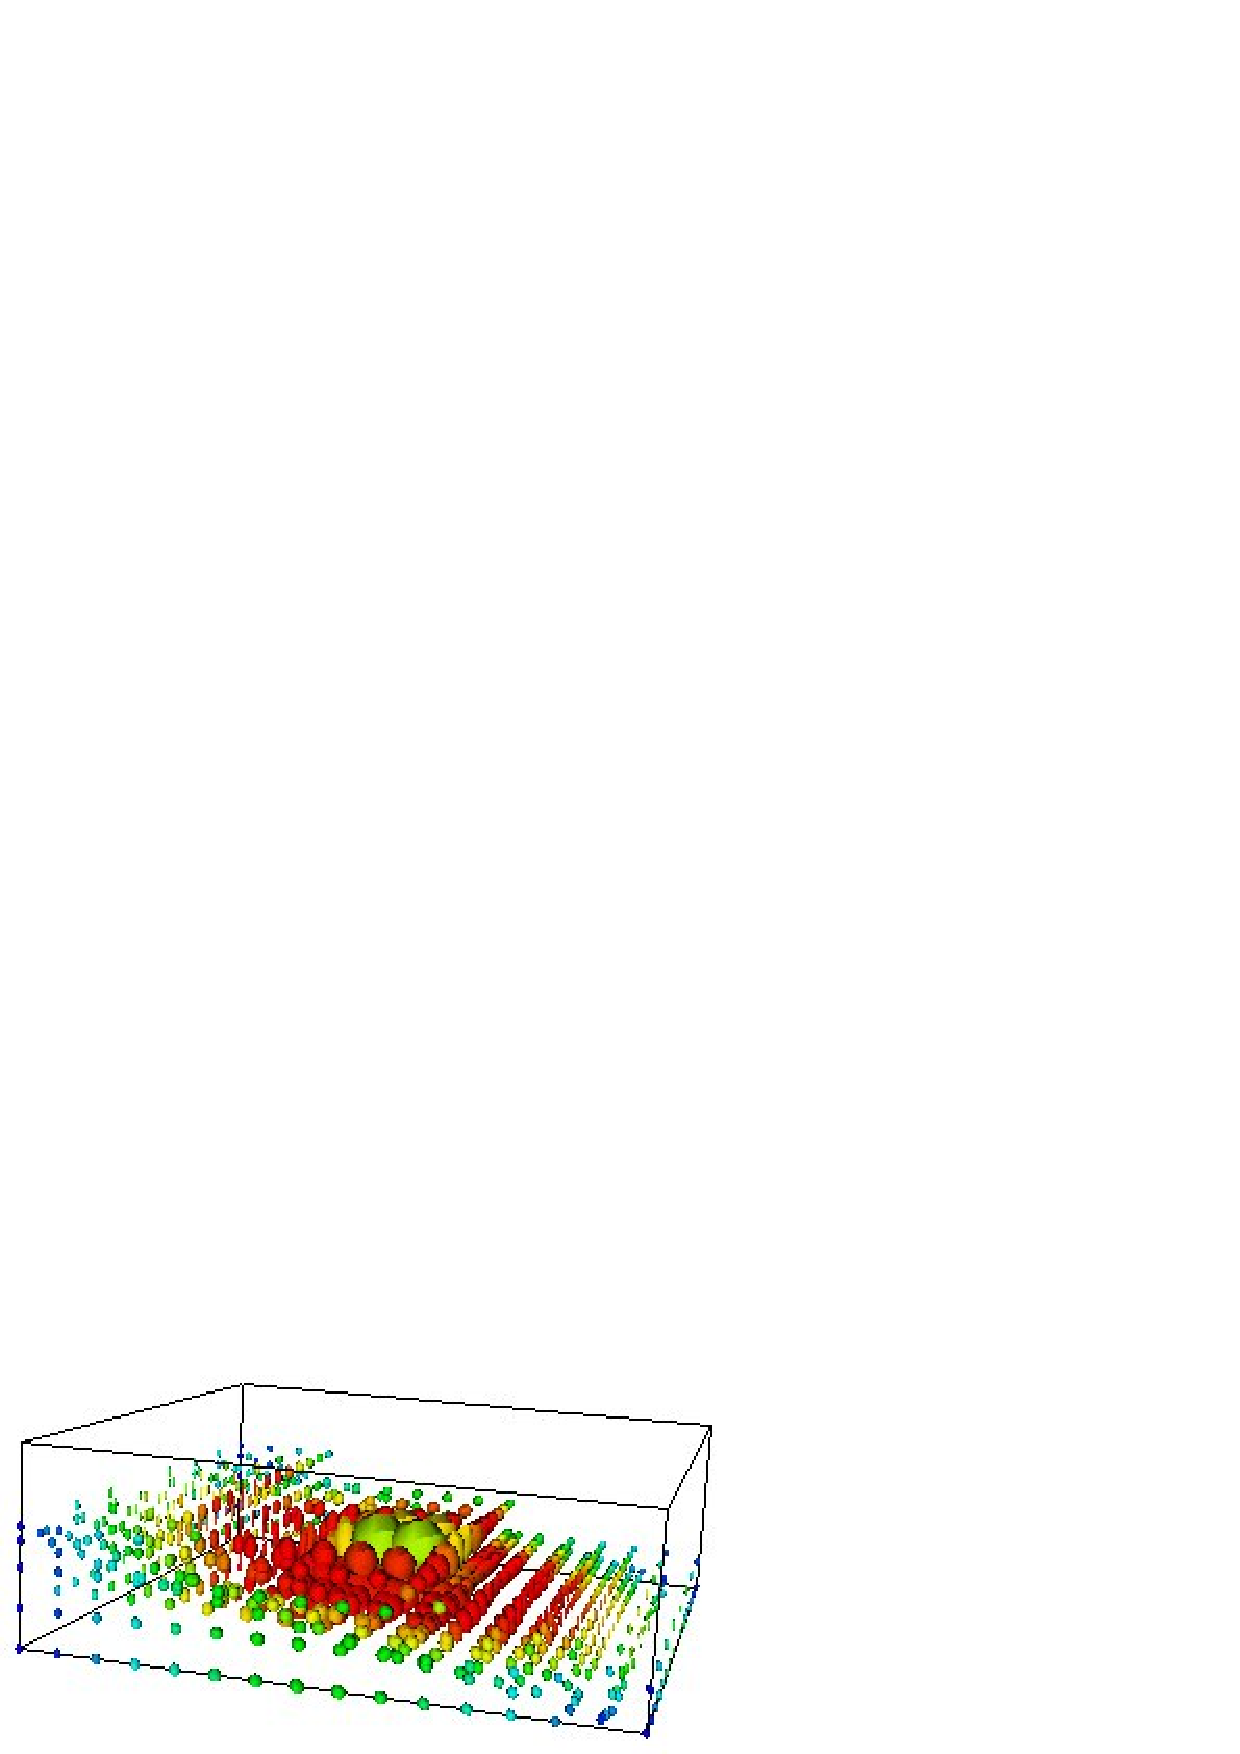
\includegraphics[width=\thumbnailwidth]{EllipsoidOnPlaneClip} \\
Ellipsoid & EllipsoidOnPlaneCut & EllipsoidOnPlaneClip \\ \\
\end{tabular}
%\caption{Sample output}
\end{table}
%
\newpage
%
\begin{table}[t]
\begin{tabular}{c c c}
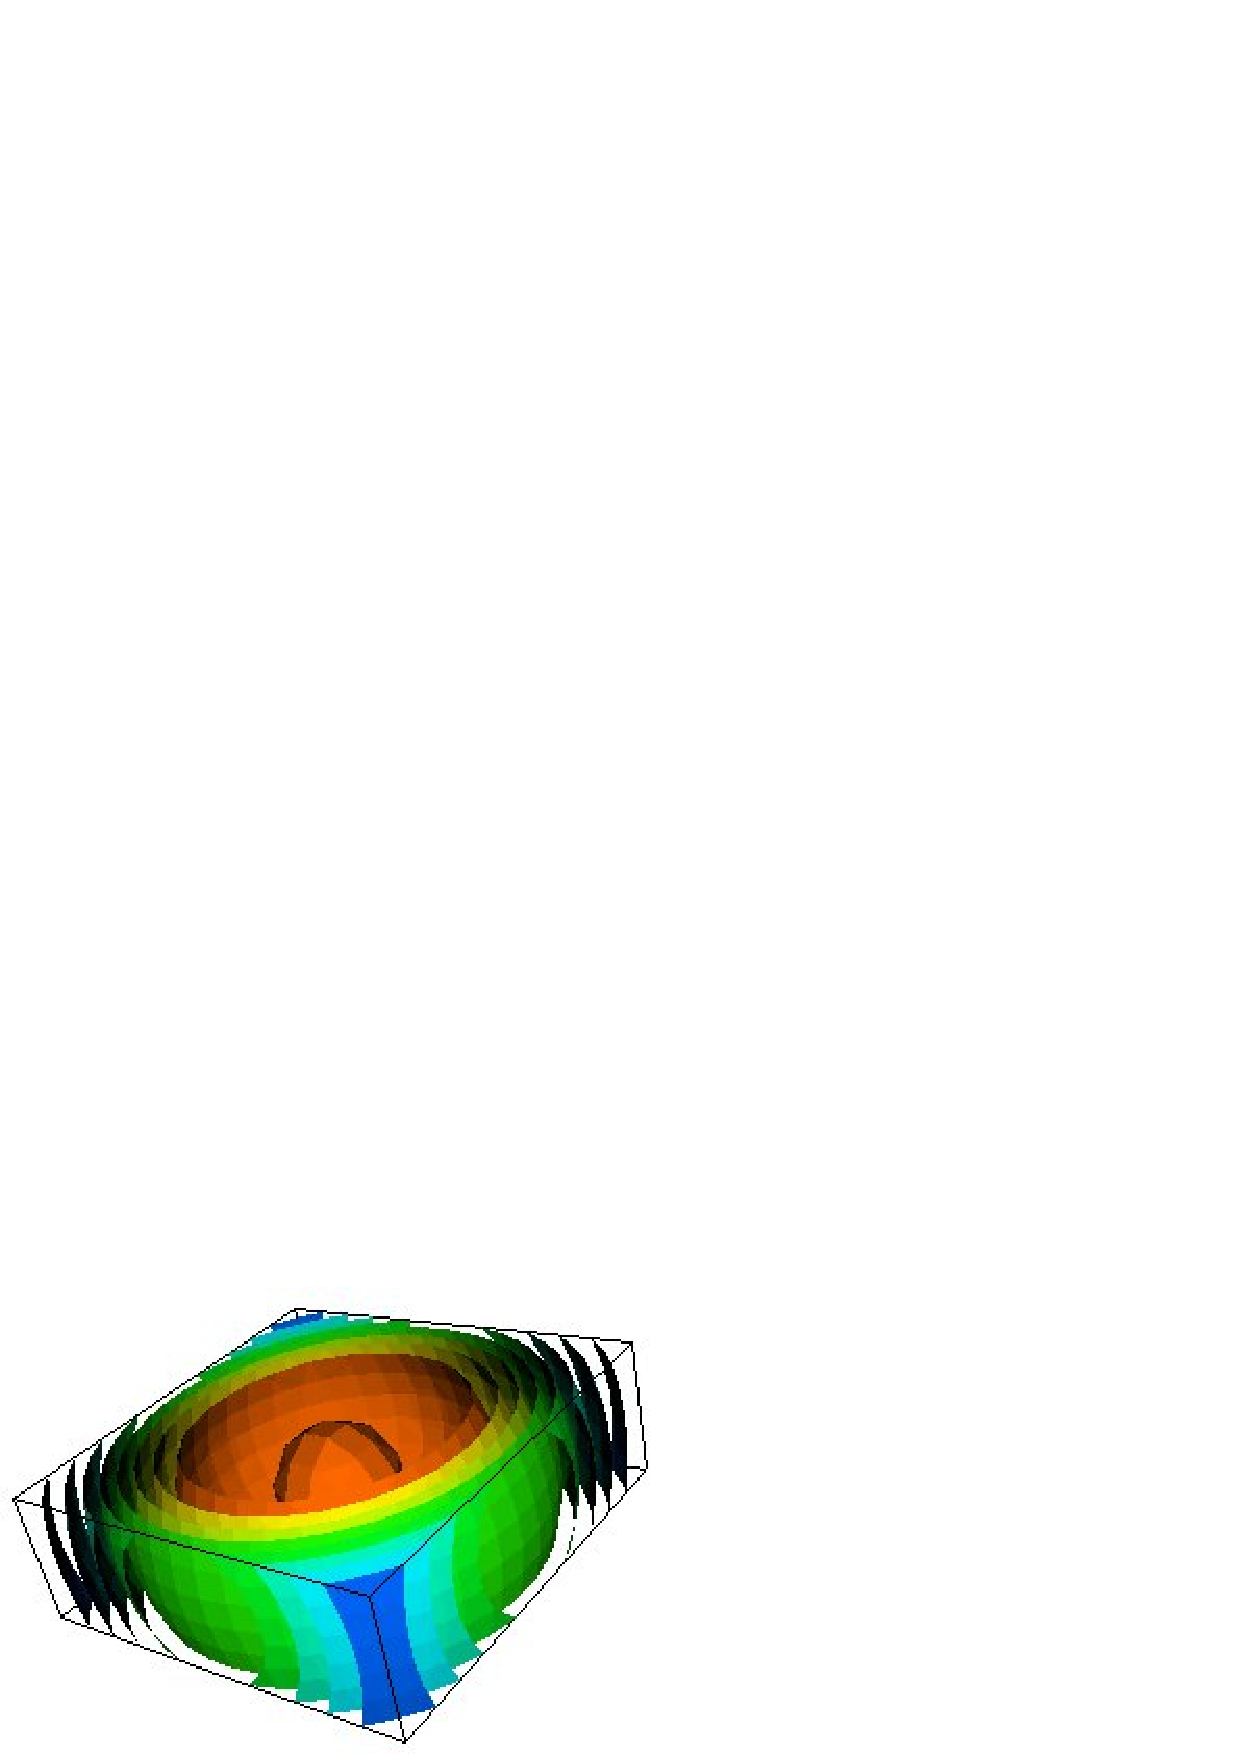
\includegraphics[width=\thumbnailwidth]{Contour} &
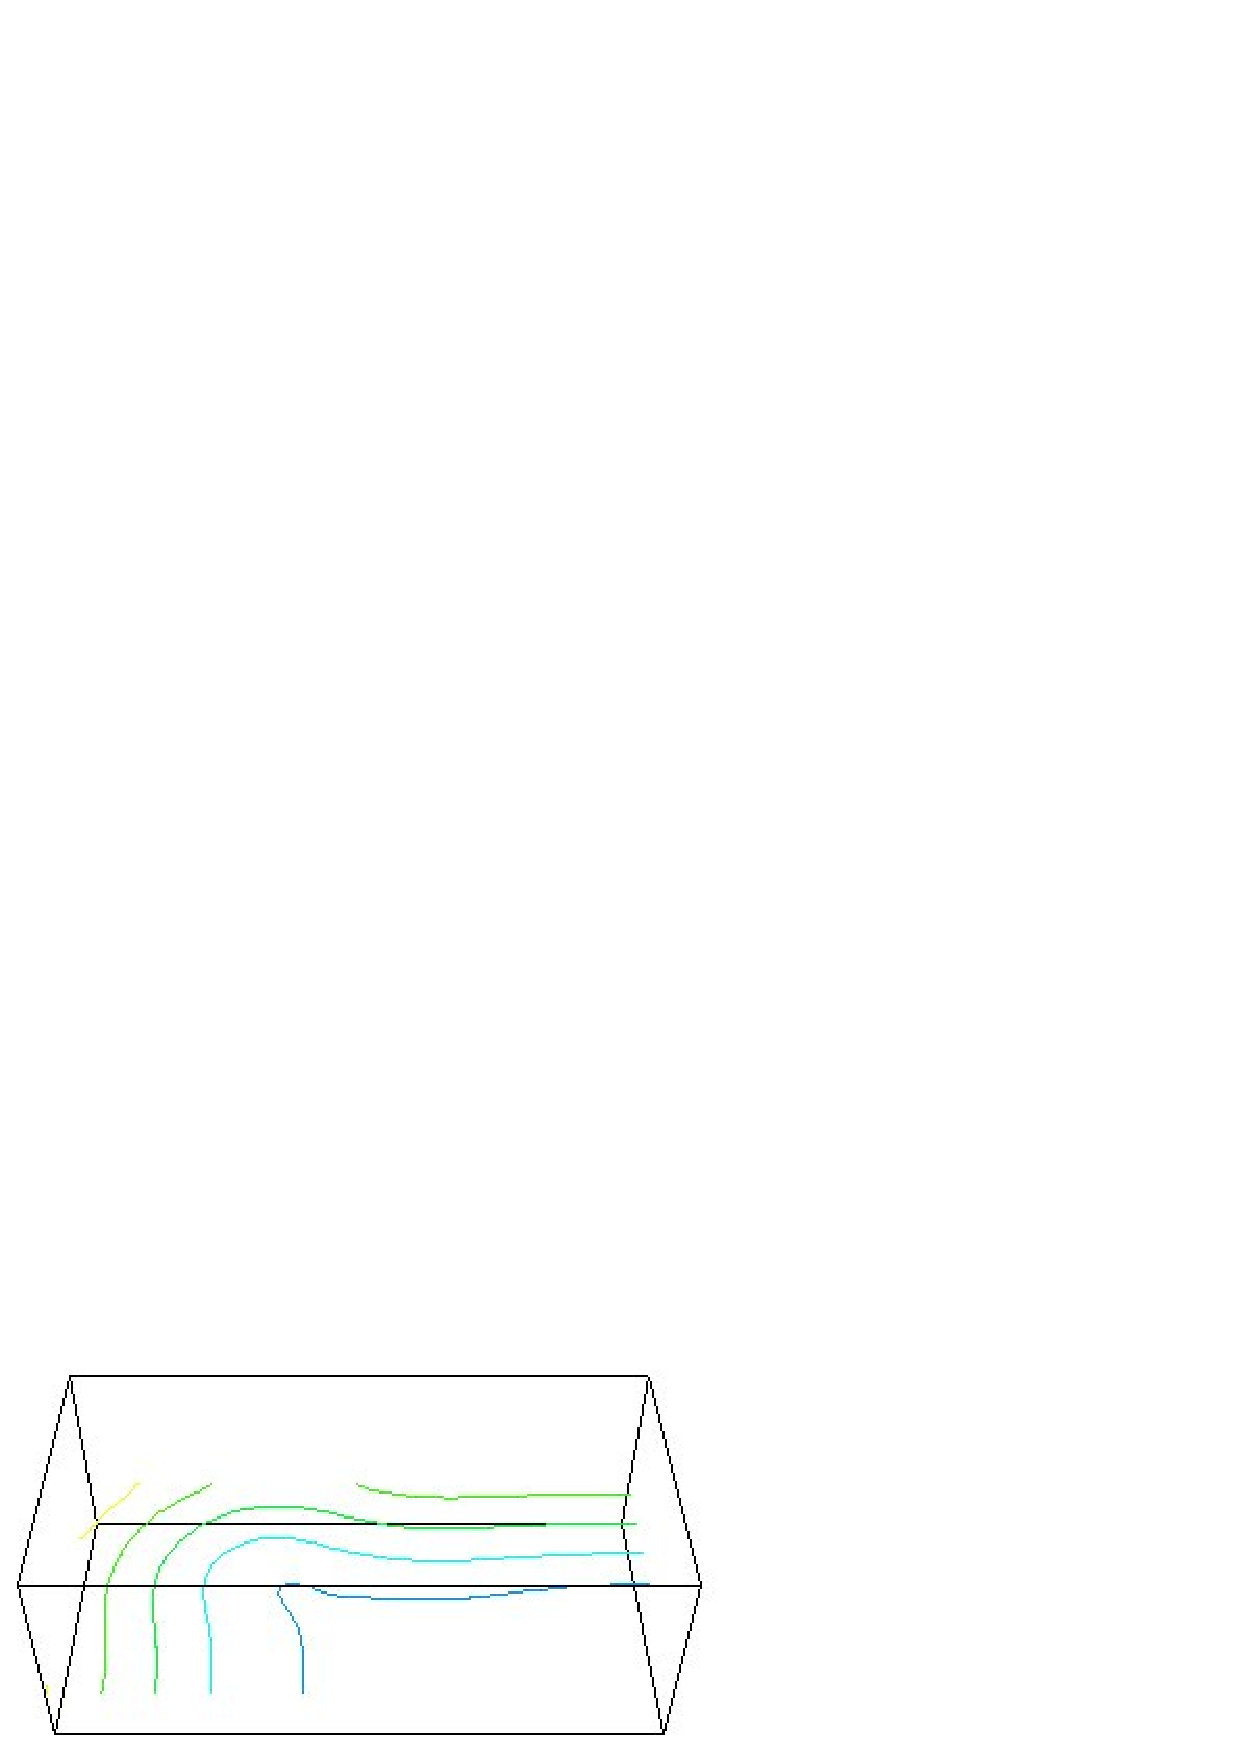
\includegraphics[width=\thumbnailwidth]{ContourOnPlaneCut} &
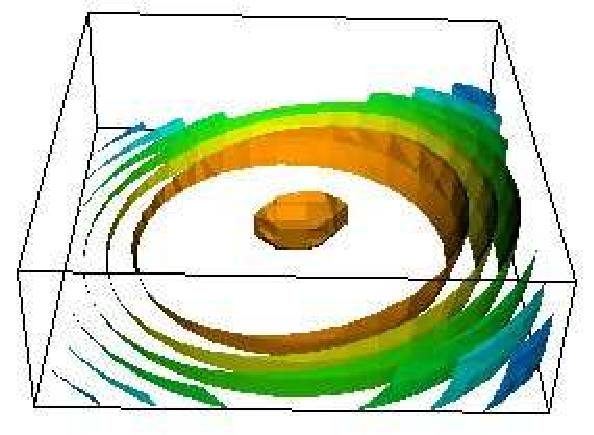
\includegraphics[width=\thumbnailwidth]{ContourOnPlaneClip} \\
Contour & ContourOnPlaneCut & ContourOnPlaneClip \\ \\ \\
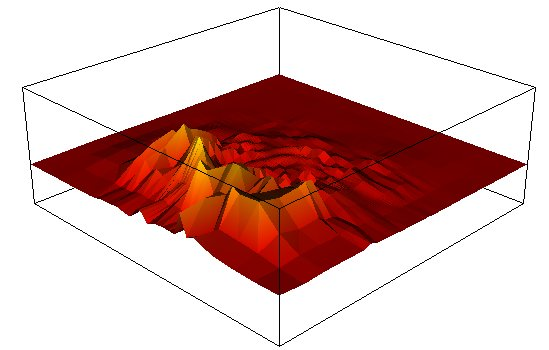
\includegraphics[width=\thumbnailwidth]{Carpet} &
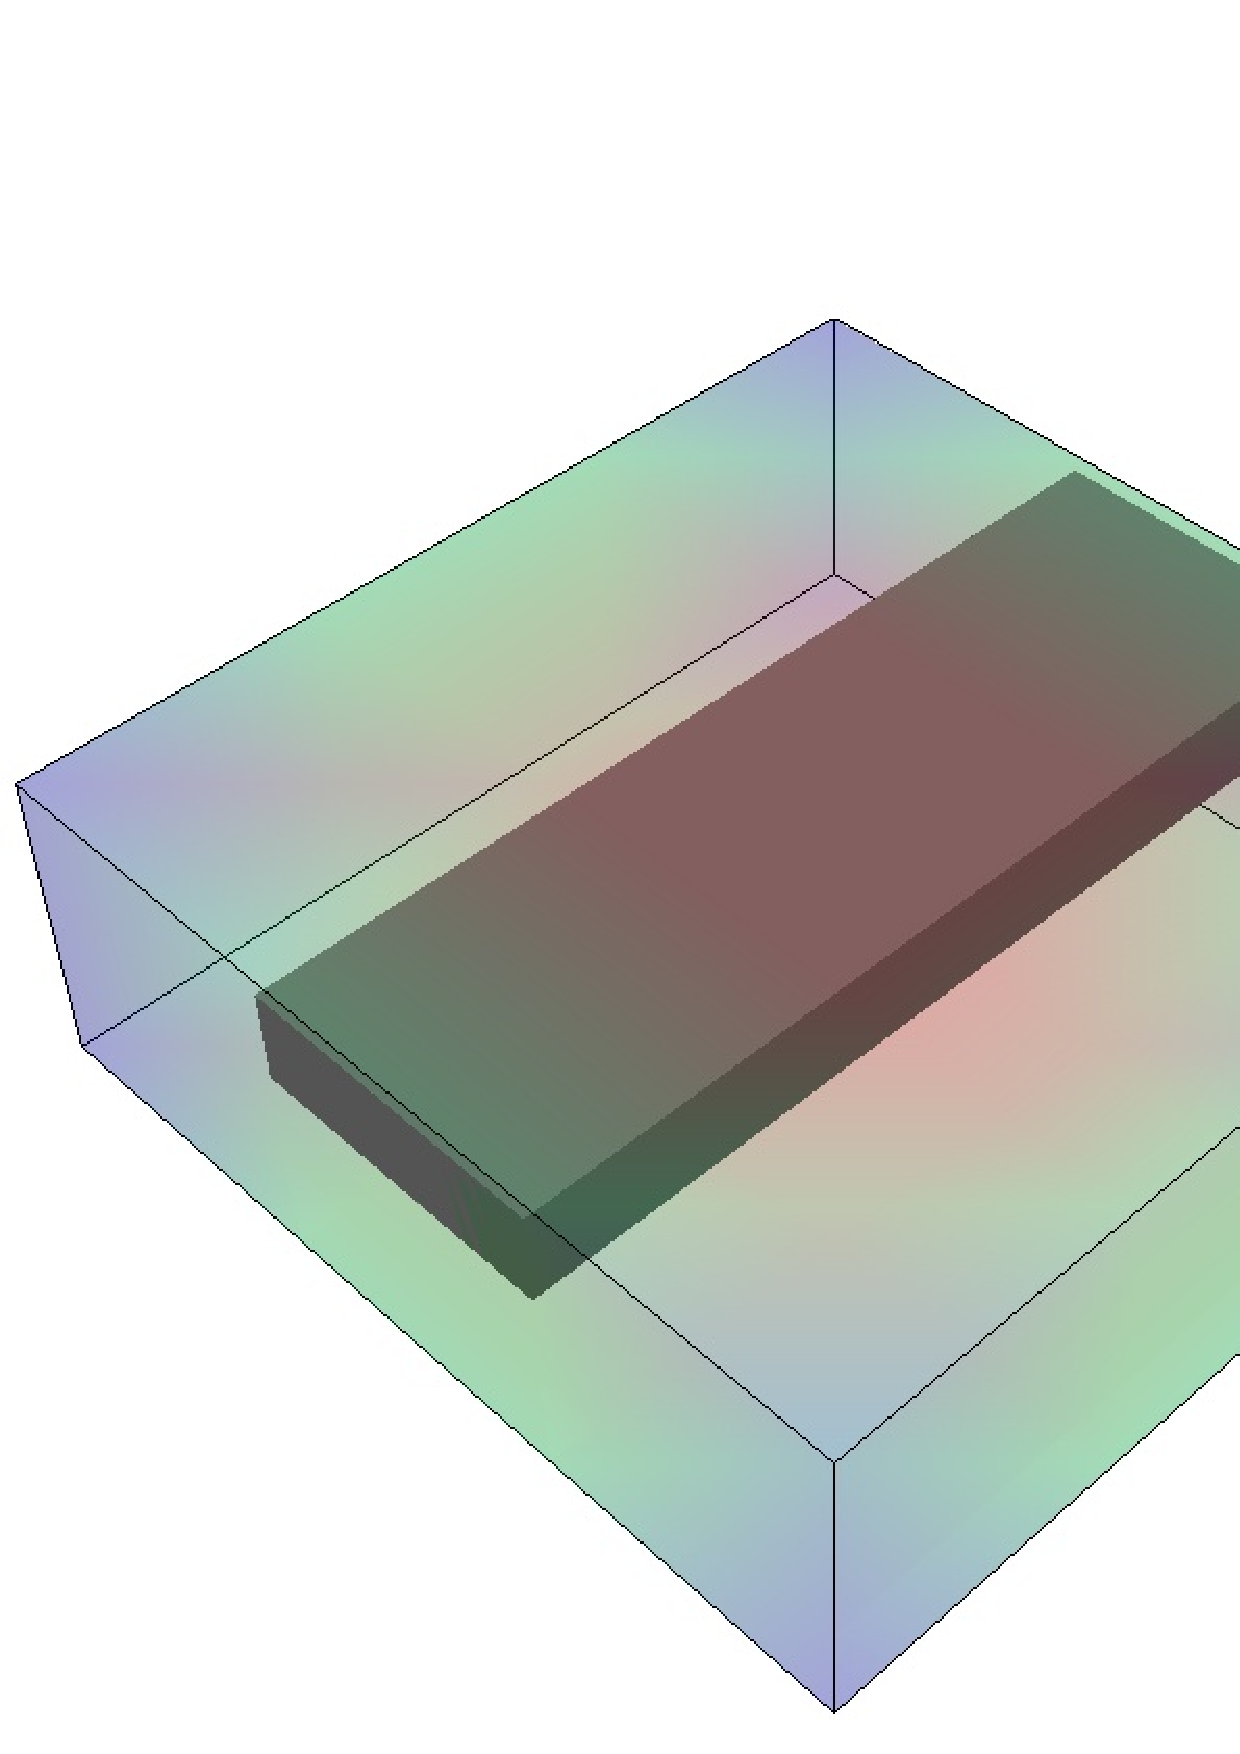
\includegraphics[width=\thumbnailwidth]{Rectangle} &
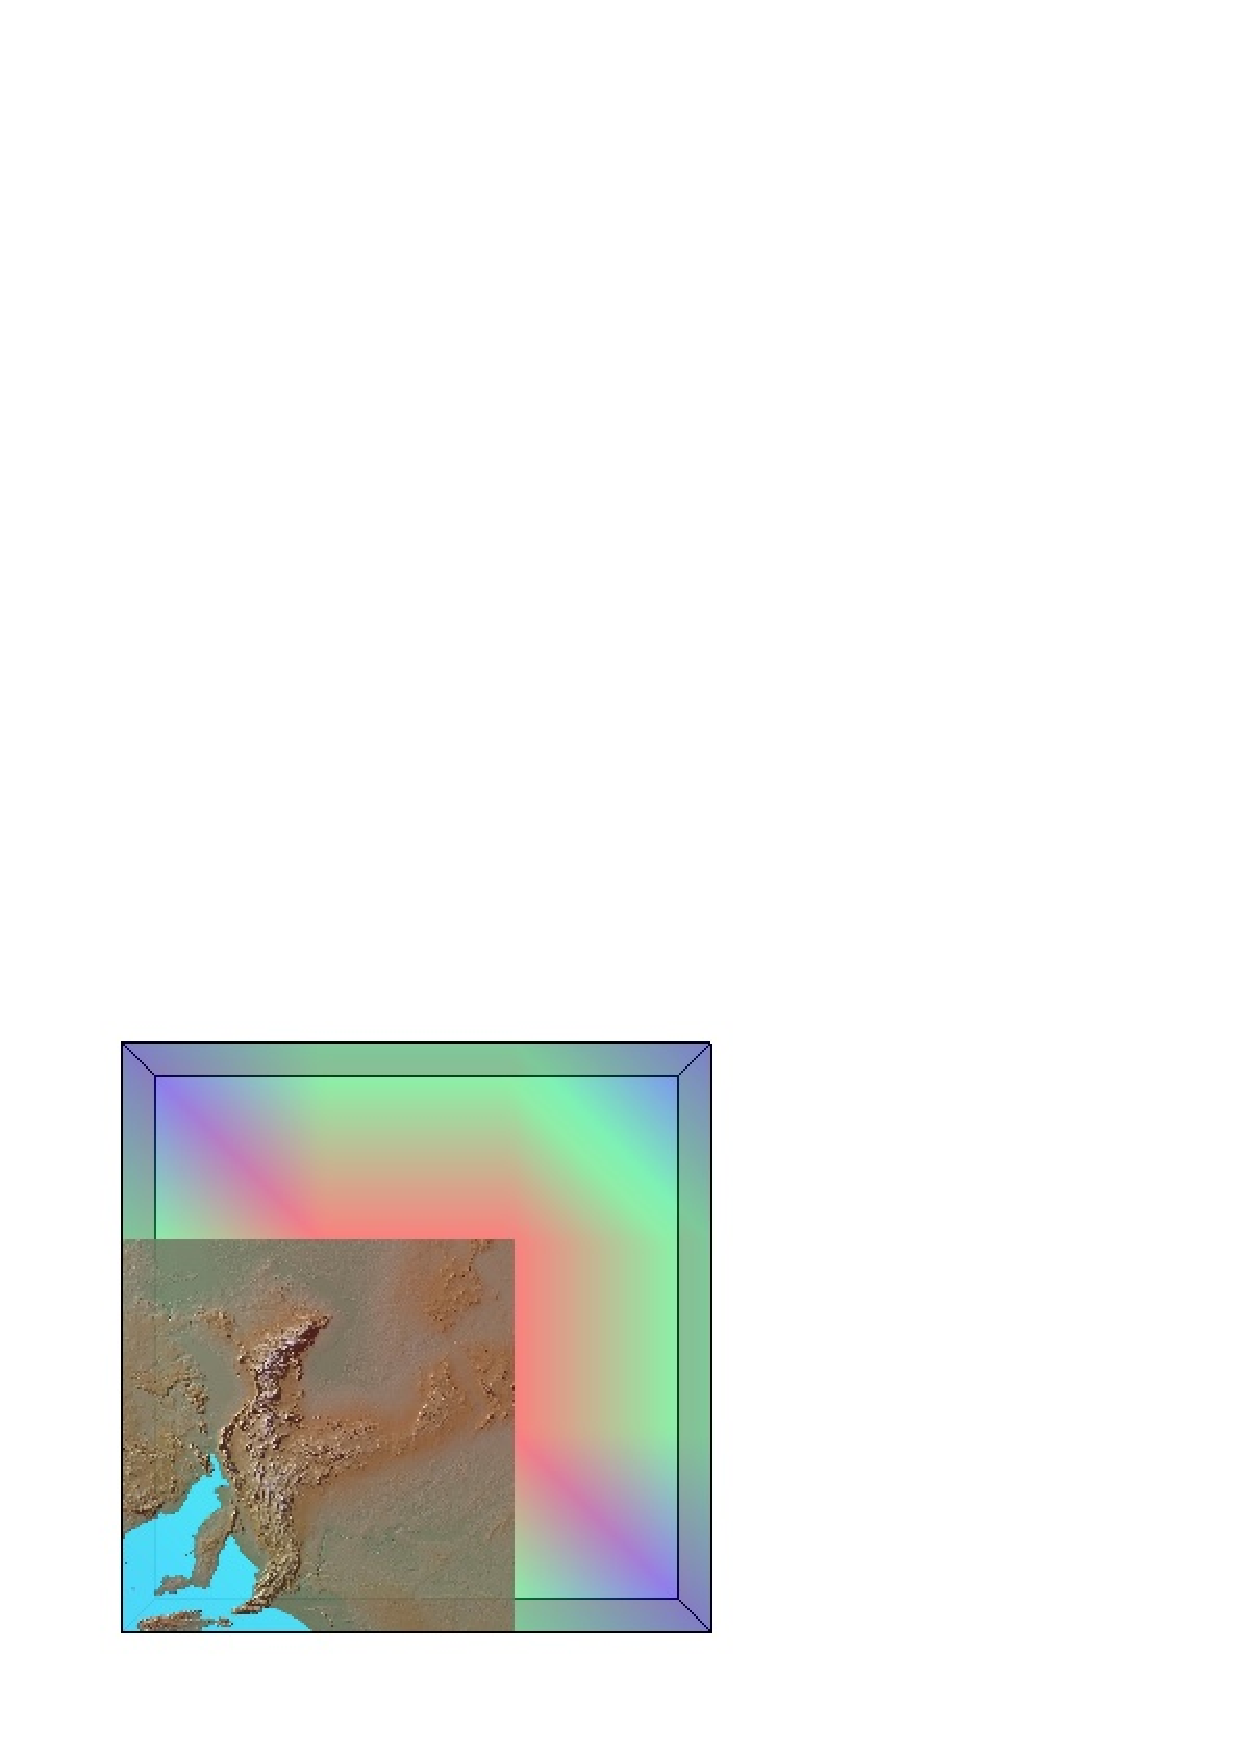
\includegraphics[width=\thumbnailwidth]{Image} \\
Carpet & Rectangle & Image \\ \\ \\ \\ \\
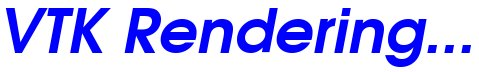
\includegraphics[width=\thumbnailwidth]{Text} &

\includegraphics[width=\thumbnailwidth]{Logo} &
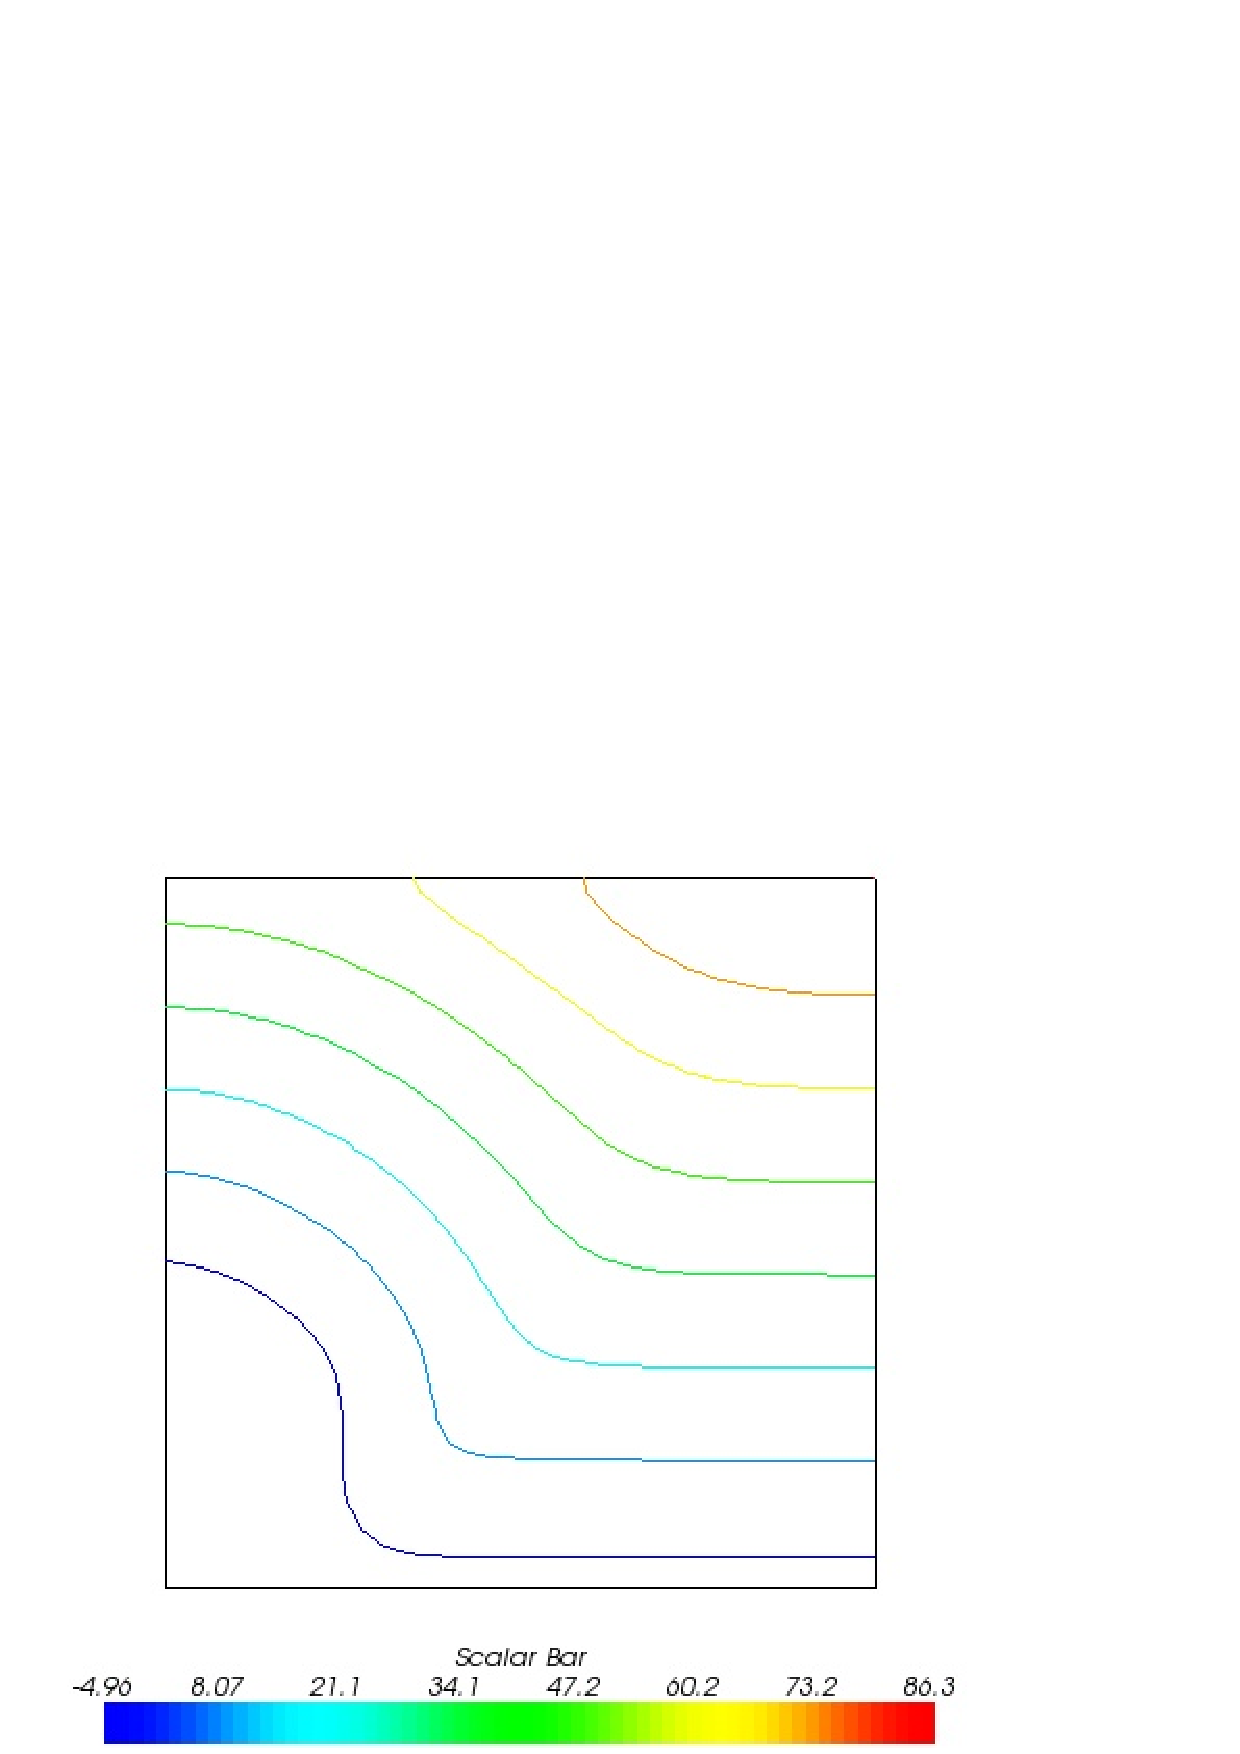
\includegraphics[width=\thumbnailwidth]{Legend} \\
Text & Logo & Legend \\ \\
\end{tabular}
%\caption{Sample Output (continued)}
\end{table}


